\chapter{Porównanie metod detekcji - eksperymenty}

Podczas eksperymentowania z~różnymi algorytmami i~metodami detekcji,
rozpoznawania obiektów oraz obróbki obrazów powstało
oraz zostało wstępnie przetestowanych wiele implementacji
najbardziej obiecujących rozwiązań. Wiele z~nich już w~trakcie
pierwszych testów prezentowało skuteczność na niezadowalającym
poziomie. Inne były zupełnie niezwiązane z~zagadnieniem,
a~jeszcze inne, choć na pierwszy rzut oka sprawiały wrażenie
wręcz niebywałe, były wysoce niestabilne.

W~tym rozdziale przedstawione i~pokrótce opisane zostały kroki podjęte
w~celu znalezienia optymalnego rozwiązania postawionego 
problemu. 
W~pierwszej kolejności zamieszczono kilka prób, które ze względu
na niezadowalające wyniki lub trudności w~implementacji
nie zostały uwzględnione w~rozwiązaniu końcowym. W~kolejnym podrozdziale
pokazano szereg prób weryfikacji skuteczności i~optymalizacji 
poszczególnych kroków ostatecznego algorytmu. W~podsumowaniu uwzględniono
częściowo przypadkowo zidentyfikowane właściwości zastosowanych
narzędzi oraz implementacji, a także wpływ tychże odkryć na
kształt finalnego rozwiązania.

\section{Algorytmy i~narzędzia nie wykorzystane w~rozwiązaniu końcowym}

W~tym podrozdziale przedstawione zostały próby, których wykonanie
skutkowało jedynie zwiększeniem świadomości na temat zagadnienia.
Główną przyczyną niewykorzystania zamieszczonych tutaj pomysłów
była niepewność co do skuteczności, bądź wydajności rozwiązania końcowego,
które miałoby być na nich oparte.

Pozostałe przyczyny to m.in. niedostosowanie rozważanego rozwiązania
do omawianego problemu. Ostatecznie zbyt duży nakład pracy, która
byłaby wymagana do dostosowania potencjalnej implementacji do
stawianych wymagań, np.: optymalizacja wysokiej złożoności obliczeniowej
lub przepisanie złożonego algorytmu na język JAVA
(w~celu uruchomienia na urządzeniu z~systemem Android)
jeżeli istniały tylko implementacje w~innych językach.

\subsection{Biblioteka OpenTLD}

Pierwszym przeciwwskazaniem do wykorzystania biblioteki OpenTLD 
był brak implementacji w~języku JAVA. Algorytm wydawał się na tyle
skomplikowany, że samo jego przeportowanie ze środowiska MatLab,
czy nawet implementacji w~C++ mogłoby stanowić zakres pracy 
inżynierskiej lub projektu zespołowego.
Pomimo to, podjęto próbę kontrolną mającą na celu sprawdzenie
skuteczności i~przydatności wspomnianego rozwiązania we wstępnej 
segmentacji - detekcji frontu autobusu - 
pierwszy krok proponowanej kaskady.

\begin{figure}[h!]
    \centering
    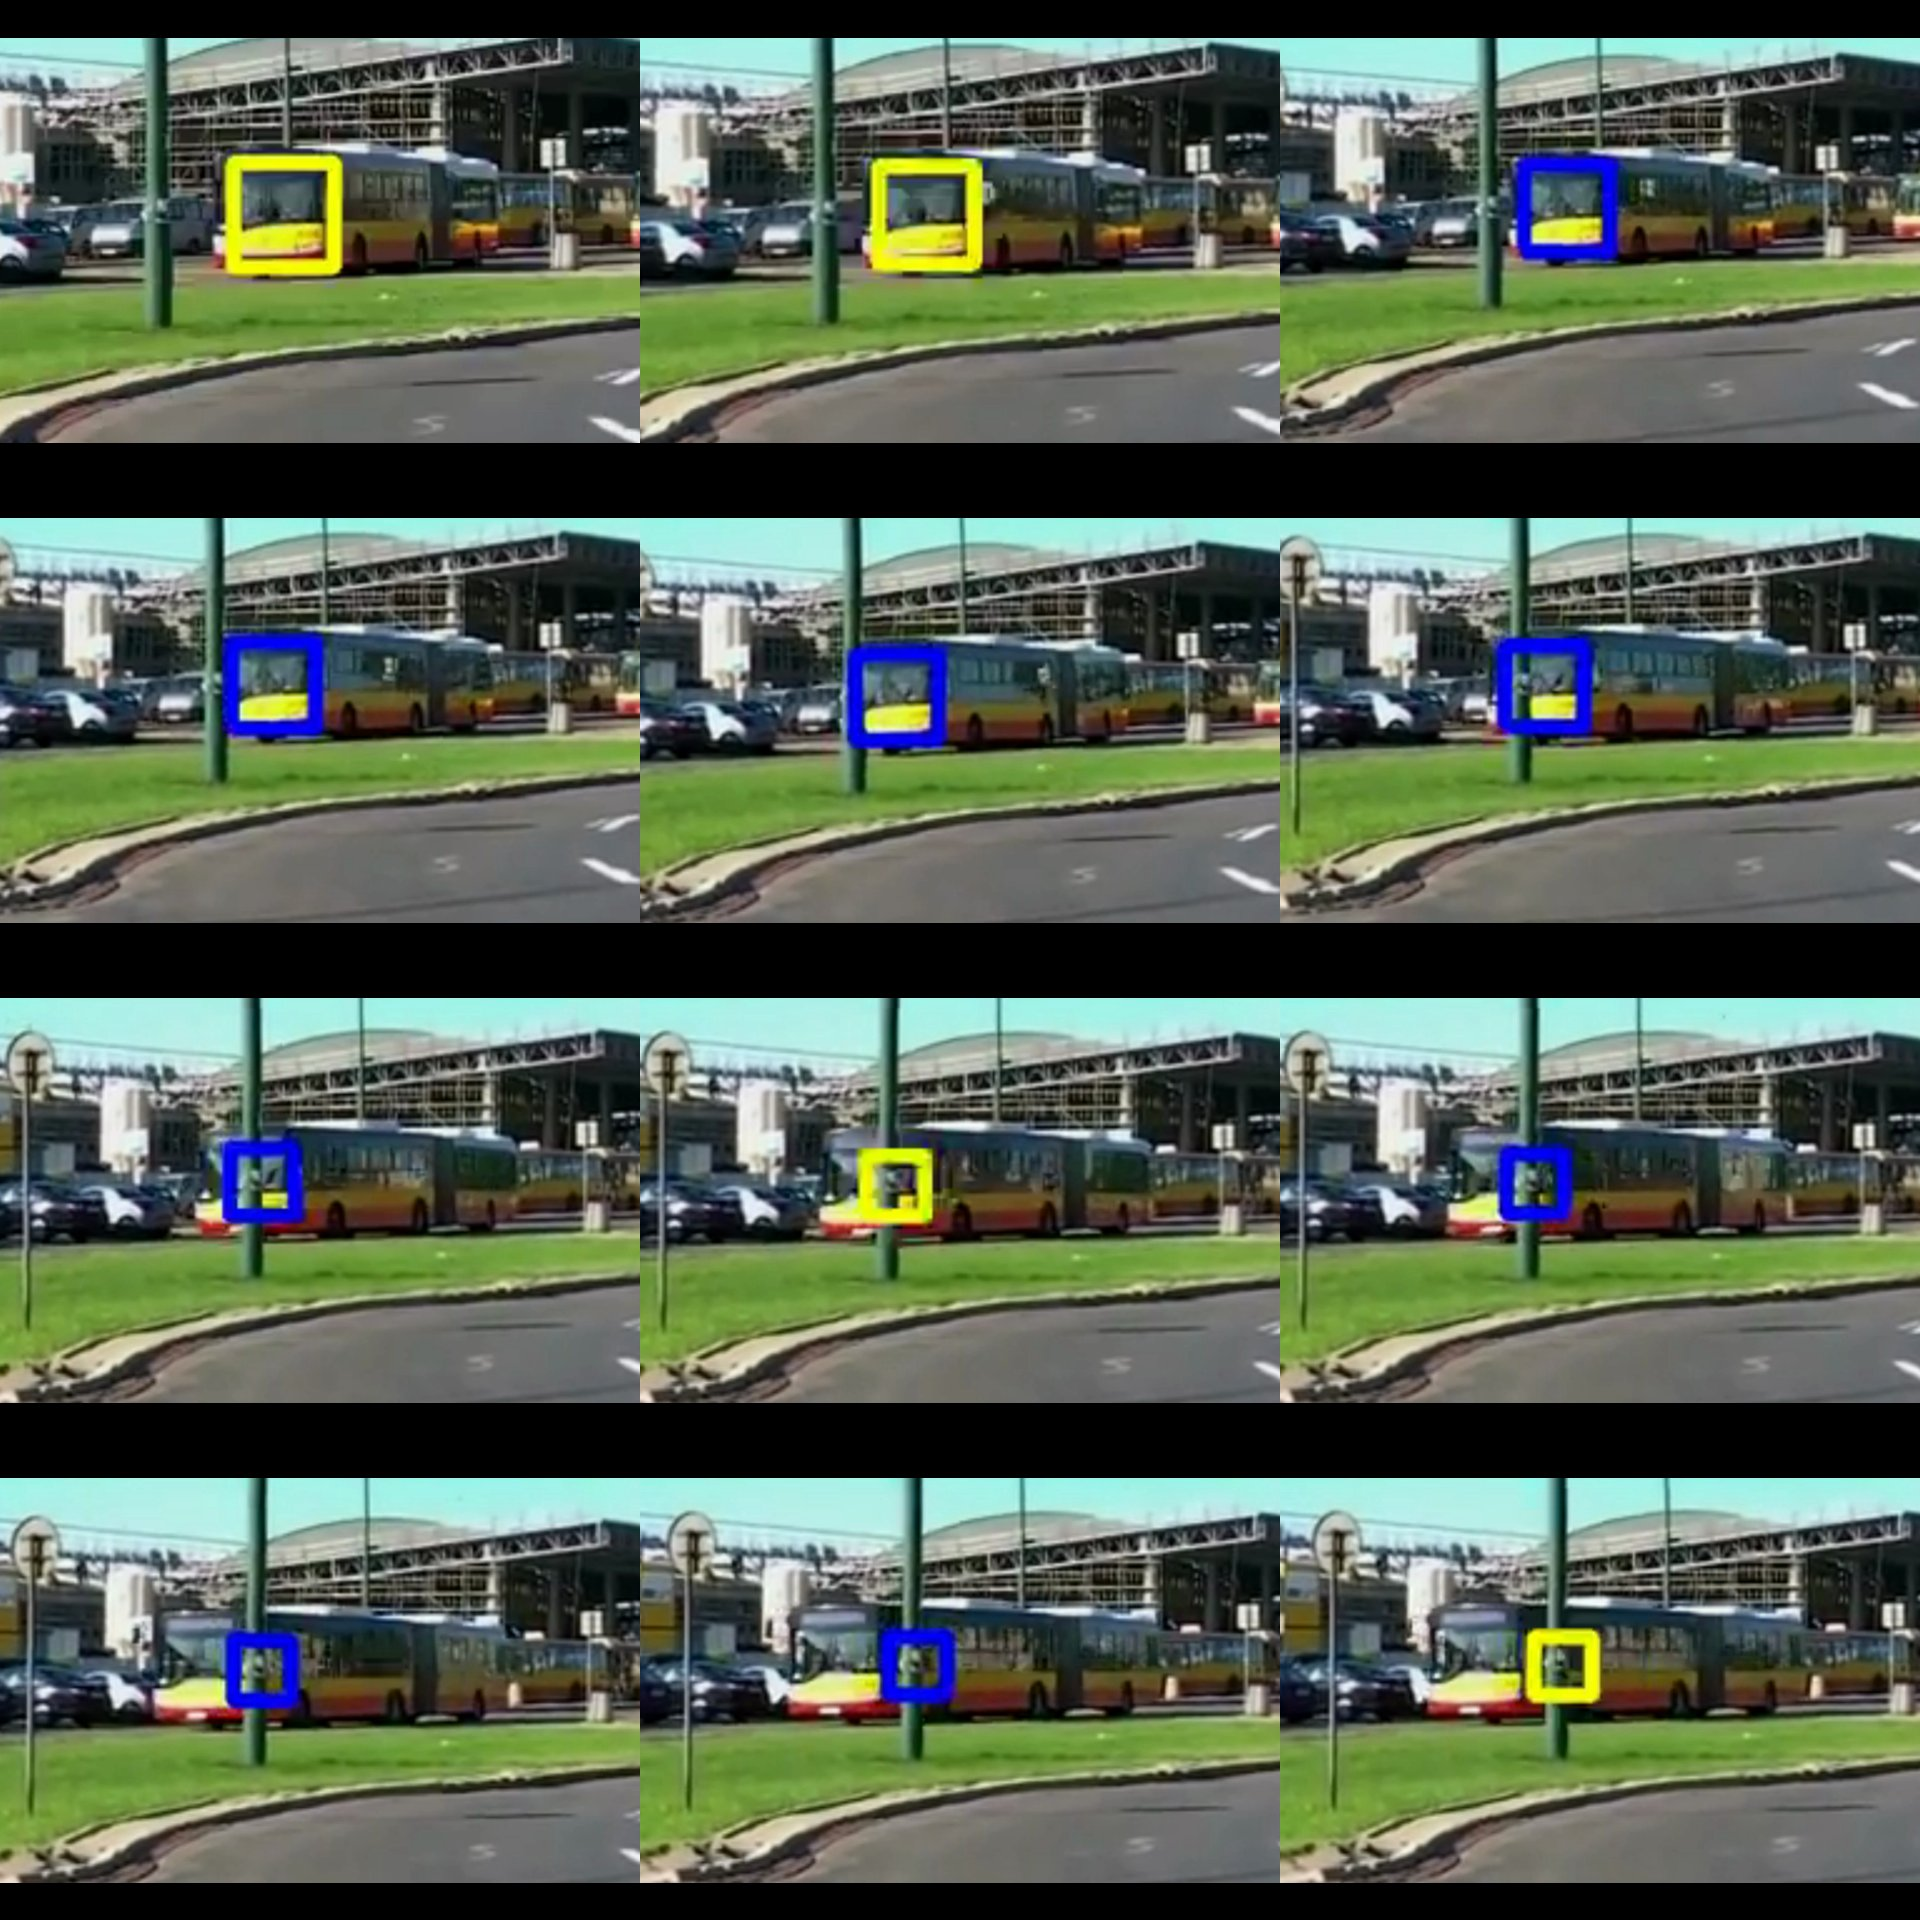
\includegraphics[width=0.9\textwidth]{img/exp_open_tld_fail}
    \caption{Niestabilność i niedokładność rezultatów uzyskanych przy
    użyciu biblioteki OpenTLD}
    \label{fig:opentld_bus_front_fail}
\end{figure}

Skuteczność wykrywania frontów autobusów (potwierdzona 
niestety jedynie w~sposób naoczny) była więcej niż zadowalająca.
Liczba trafień uzyskanych z~pojedynczego wstępnego zaznaczenia frontu
była niemal stuprocentowa. Niestety dokładność wykrytych obiektów
była poniżej oczekiwanej. Standardowo zdarzały się problemy
obciętych numerów - zbyt mały czworokąt okalający. Dodatkowo
brak możliwości ingerencji w~proces uczenia detektora oraz jego
duże tendencje do ,,pływania'' skutkowały nieraz wynikami pozytywnymi
typu: lewy dolny róg frontu do 1/2 wysokości i~szerokości. 

Na rysunku \ref{fig:opentld_bus_front_fail} można zaobserwować 
zupełne zgubienie obiektu 
śledzonego - 
front autobusu - na rzecz słupa. Wynik tego eksperymentu oraz
zaobserwowany spadek wydajności - liczby obsłużonych klatek na sekundę - 
dla rosnącej liczby zebranych pozytywnych i~negatywnych próbek
(na powyższym rysunku żółte kwadraty oznaczają próbkę, która została
wykorzystana do procesu uczenia detektora) 
wpłynęły na decyzję o~zaprzestaniu dalszych testów biblioteki OpenTLD.
Ostatecznie dla jednej sesji,
nagrania długości około 5 minut, wydajność potrafiła spaść z~poziomu
początkowych 20 klatek na sekundę do nawet 2 klatek na sekundę.
Poprawa tego stanu 
rzeczy wykracza poza zakres niniejszej pacy. Szczególnie, że Pan 
Zdenek Kalal wydał drugą wersję biblioteki TLD (tym razem już nie 
open), której jednym z~głównych usprawnień był właśnie znaczny 
wzrost wydajności
\cite{WEB:kalaltld2}.

\subsection{Wykrywanie linii krawężnika zatoki autobusowej}

Po podjęciu decyzji o~rezygnacji
z~wykorzystania
biblioteki OpenTLD, w~ramach poszukiwań optymalnego sposobu wstępnej
segmentacji użyty został filtr ,,Canny'' z~pakietu OpenCV. Celem prac
miał być detektor krawędzi, który mógłby zostać użyty do
wykrycia górnej krawędzi frontu autobusu lub zarysu autobusu w~ogóle.
Po wykryciu bliżej niezdefiniowanego zestawu pionowych i~poziomych
krawędzi oraz zastosowaniu co do niego takich samych (bliżej
niezdefiniowanych) ograniczeń geometrycznych, algorytm miałby
stwierdzić, że fragment którego cechy spełniają pewne kryteria jest
właśnie frontem autobusu.

Patrząc na kilka wynikowych obrazów reprezentujących wykryte krawędzie,
okazało się, że najlepiej 
widoczną linią (krawędzią) jest linia wyznaczona przez krawężnik
zatoki autobusowej.

\begin{figure}[h!]
    \centering
    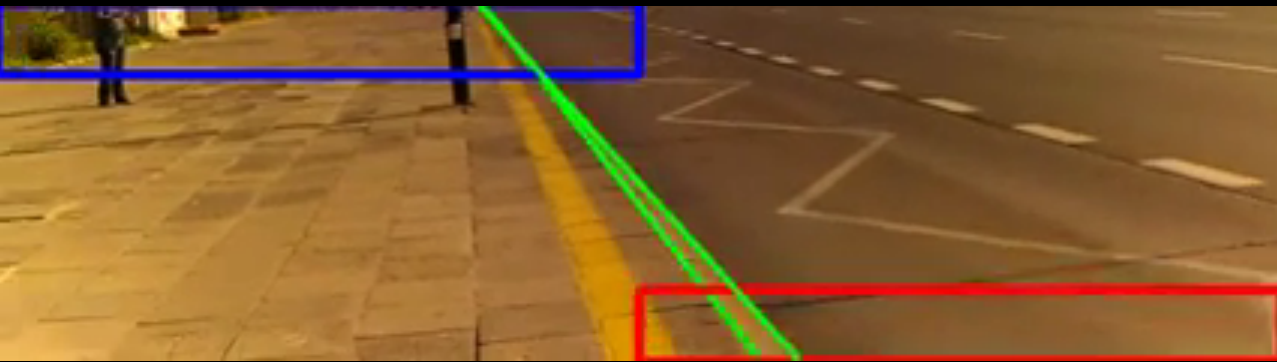
\includegraphics[width=0.9\textwidth]{img/exp_bus_lane_edge_detector}
    \caption{Wykrywacz linii krawędzi zatoki autobusowej}
    \label{fig:bus_lane_edge_detection}
\end{figure}

Rysunek \ref{fig:bus_lane_edge_detection} przedstawia wynik 
eksperymentalnej wersji programu do
wykrywania krawędzi zatoki autobusowej. W~implementacji użyty
został prosty ,,Canny edge detector''. Zakładając, że osoba stojąca
na przystanku jest skierowana twarzą (kamerą) do nadjeżdżającego autobusu,
linia wyznaczona przez krawężnik zatoki powinna zaczynać się w~połowie
wysokości klatki (obraz na powyższym rysunku przedstawia jej dolną
połowę) bardziej z~lewej strony - niebieski prostokąt. Koniec linii
powinien znajdować się na dole klatki bardziej z~prawej strony - czerwony
prostokąt.

Zrezygnowano z~tego pomysłu ze względu na zbyt dużą ilość 
specyficznych
ograniczeń geometrycznych i~niezamierzoną dyskryminację pasażerów
których zatoki przystankowe nie mają krawężników. Ostatnim argumentem
na niekorzyść, 
byli inni pasażerowie stojący na przystanku, którzy
zasłaniali krawężnik na przystanku czyniąc tę metodę bezużyteczną.

Na tym etapie podjęta została decyzja, że wstępna segmentacja
zostanie wykonana przy użyciu kaskadowego detektora cech (HAAR, HOG, LBP)
opisana w~artykule autorstwa Viola i~Jonesa \cite{DBLP:conf/cvpr/ViolaJ01}.

\subsection{Progowanie HSV}

Równoległym pomysłem do kaskadowego detektora było 
wykorzystanie progowania obrazu w~dziedzinie HSV (\textit{
ang. Hue Saturation Value})
w~celu wyodrębnienia wyświetlacza z~numerem linii. 
Kolejne niepokojące założenie, które poczyniono
na wstępnym etapie prac, dotyczyło koloru numeru linii autobusowej.
Przyjęto, że odcień numeru będzie (w~znacznej ilości przypadków) 
zbliżony do pomarańczowego - z~możliwością rozszerzenia o~kolor
zielony. 

\begin{figure}[h!]
    \centering
    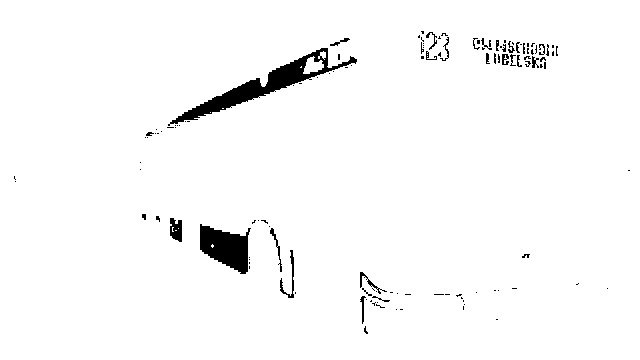
\includegraphics[width=0.9\textwidth]{img/exp_hsv_threshold_number_detector}
    \caption{Segmentacja numeru metodą progowania HSV}
\end{figure}

Po wykryciu potencjalnego numeru należałoby uruchomić drugi stopień
kaskady, który stwierdzałby czy dany fragment rzeczywiście reprezentuje
numer.

Niestety niepewność związana z~niepożądanym wykrywaniem przypadkowych
pomarańczowych numerów i~dyskryminacją pasażerów, którzy
poruszają się autobusami z~zielonymi wyświetlaczami skutecznie
zniechęciła do implementacji rzeczonego rozwiązania.

Na tym etapie dodatkowym argumentem było niepożądane 
pominięcie w~ten sposób
wszystkich autobusów z~tabliczkami gdzie numer zapisywany jest czarną
czcionką na białym tle. Argument ten był jeszcze wtedy aktualny, choć
ostatecznie zrezygnowano z~wykrywania frontów tzw. ,,starego typu'' -
Ikarus, Jelcz Berliet itp. Zostało to pośrednio wymuszone przez 
znacznie mniejszą skuteczność uniwersalnego detektora, który był
wyszkolony przy użyciu frontów z~tabliczkami i~tych z~wyświetlaczami, 
o~czym szerzej w~podrozdziale \ref{sec:testynarzedziwykorzystanych}.

\subsection{Gotowy silnik OCR - Tesseract}

Pierwsza próba z~narzędziem Tesseract okazała się bardzo obiecująca.
Ręcznie wycięty fragment reprezentujący numer 140 został podany 
jako argument wywołania komendy \verb|tesseract|:

\lstinputlisting{data/tesseractcommand.txt}

Parametr \verb|-psm 8| określał metodę segmentacji obrazu jako ,,jedno
słowo''. Obraz wejściowy \verb|number.png| został zaprezentowany
na rysunku \ref{fig:sample_tesseract_input}. Wynik jaki otrzymano dla 
powyższego doświadczenia
był wzorowy - w~pliku wynikowym \verb|out.txt| pojawił
się oczekiwany ciąg znaków (104).

\begin{figure}[h!]
    \centering
    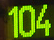
\includegraphics[width=0.25\textwidth]{img/exp_number_01}
    \caption{Pierwszy numer testowy - prawidłowo odczytany}
    \label{fig:sample_tesseract_input}
\end{figure}

Szereg kolejnych doświadczeń przyniósł jednak rozczarowanie. 
Wiele dobrze widocznych numerów w~stosunkowo wysokiej rozdzielczości 
nie zostało odczytanych w~ogóle (ciąg znaków zerowej długości). Zdarzały 
się nawet przypadki, kiedy trzycyfrowy numer został rozszyfrowany jako
kilka wielocyfrowych liczb (ciąg ze spacjami).

\begin{table}[h!]
  \centering
  \caption{Wyniki pierwszej serii testowej Tesseract}\label{tbl:tess_01}
  \begin{tabular}{| c | l | c | l | c | l |}
  	\hline
    Obraz & Odczyt & Obraz & Odczyt & Obraz & Odczyt  \\ 
    \hline
    \begin{minipage}{.2\textwidth}
      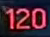
\includegraphics[width=\textwidth]{img/exp_number_02}
    \end{minipage}
    &
    '120'
    &
    \begin{minipage}{.2\textwidth}
      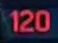
\includegraphics[width=\textwidth]{img/exp_number_03}
    \end{minipage}
    &
    '120.'
    &
    \begin{minipage}{.2\textwidth}
      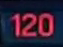
\includegraphics[width=\textwidth]{img/exp_number_04}
    \end{minipage}
    &
    '120'
    \\
    \hline
    \begin{minipage}{.2\textwidth}
      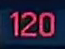
\includegraphics[width=\textwidth]{img/exp_number_05}
    \end{minipage}
    &
    '120'
    &
    \begin{minipage}{.2\textwidth}
      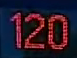
\includegraphics[width=\textwidth]{img/exp_number_06}
    \end{minipage}
    &
    '120'
    &
    \begin{minipage}{.2\textwidth}
      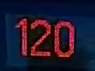
\includegraphics[width=\textwidth]{img/exp_number_07}
    \end{minipage}
    &
    '120'
    \\ 
    \hline
  \end{tabular}
\end{table}

Niestety w~momencie pisania tego tekstu wyniki pierwotnych eksperymentów
zostały utracone. Mając już gotową implementację opartą na innym
rozwiązaniu wykonano dwie krótkie serie próbne, których wyniki
zamieszczono w~tabelach \ref{tbl:tess_01}, \ref{tbl:tess_02} i \ref{tbl:tess_03}.

Pierwsza seria próbna pokazuje, że rozwiązanie oparte na narzędziu
Tesseract ma duży potencjał i~wysokie prawdopodobieństwo powodzenia.
Jednak, aby zobrazować problemy jakie niesie ze sobą to podejście,
wykonano dwie kolejne, celowo nieudane próby.

\begin{table}[h!]
  \centering
  \caption{Wyniki drugiej serii testowej Tesseract}\label{tbl:tess_02}
  \begin{tabular}{| c | l | c | l |}
  	\hline
    Obraz & Odczyt & Obraz & Odczyt  \\ 
    \hline
    \begin{minipage}{.2\textwidth}
      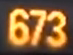
\includegraphics[width=\textwidth]{img/exp_number_n01}
    \end{minipage}
    &
    '673'
    &
    \begin{minipage}{.2\textwidth}
      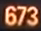
\includegraphics[width=\textwidth]{img/exp_number_n02}
    \end{minipage}
    &
    '673'
     
    \\ 
    \hline

    \begin{minipage}{.2\textwidth}
      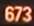
\includegraphics[width=\textwidth]{img/exp_number_n03}
    \end{minipage}
    &
    '673'
    &
    \begin{minipage}{.2\textwidth}
      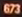
\includegraphics[width=\textwidth]{img/exp_number_n04}
    \end{minipage}
    &
    '.'

    \\ 
    \hline

  \end{tabular}
\end{table}

W~drugiej serii przedstawiono zależność skuteczności Tesseracta od 
rozdzielczości obrazu, gdzie czwarty obraz został zinterpretowany
jako kropka. Poziom dokładności jest w~tym przypadku na poziomie
jak najbardziej akceptowalnym. Trudno nawet spodziewać się lepszego
wyniku.

Największe wątpliwości
co do wykorzystania Tesseracta w~rozwiązaniu docelowym zostały zobrazowane
przez wyniki trzeciej serii testowej. Tutaj zniekształcenia spowodowane
refleksami pojawiającymi się na szybie osłaniającej wyświetlacz
zupełnie uniemożliwiły skuteczne odczytanie numeru.

\begin{table}[h!]
  \centering
  \caption{Wyniki trzeciej serii testowej Tesseract}\label{tbl:tess_03}
  \begin{tabular}{ | c | l | c | l | c | l | }
  	\hline
    Obraz1 & Odczyt1 & Obraz2 & Odczyt2 & Obraz3 & Odczyt3  \\ 
    \hline
    \begin{minipage}{.2\textwidth}
      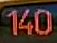
\includegraphics[width=\textwidth]{img/exp_number_f01}
    \end{minipage}
    &
     '26'
    &
    \begin{minipage}{.2\textwidth}
      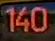
\includegraphics[width=\textwidth]{img/exp_number_f02}
    \end{minipage}
    &
    '170'
    &
    \begin{minipage}{.2\textwidth}
      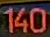
\includegraphics[width=\textwidth]{img/exp_number_f03}
    \end{minipage}
    &
    '140'
    \\
    \hline
    \begin{minipage}{.2\textwidth}
      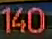
\includegraphics[width=\textwidth]{img/exp_number_f04}
    \end{minipage}
    &
    ' 9.'
    &
    \begin{minipage}{.2\textwidth}
      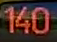
\includegraphics[width=\textwidth]{img/exp_number_f05}
    \end{minipage}
    &
     brak
    &
    \begin{minipage}{.2\textwidth}
      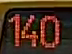
\includegraphics[width=\textwidth]{img/exp_number_f06}
    \end{minipage}
    &
     brak
    \\
    \hline
    \begin{minipage}{.2\textwidth}
      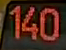
\includegraphics[width=\textwidth]{img/exp_number_f07}
    \end{minipage}
    &
     '1420.'
    &
    \begin{minipage}{.2\textwidth}
      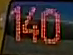
\includegraphics[width=\textwidth]{img/exp_number_f08}
    \end{minipage}
    &
     '711913'
    &
    &
    \\
    \hline

  \end{tabular}
\end{table}

Dodatkowym problemem była prawdopodobna tendencja do nadinterpretacji
przy odczycie numerów gdy rozdzielczość była już na tyle wysoka, że
widoczne były poszczególne diody - ostatni obraz z~serii trzeciej.
Rozwiązaniem tego problemu byłoby zastosowanie adaptacyjnego filtru
Gaussa lub operacji morfologicznych, np.: otwarcia + zamknięcia.
Opór przed tego typu zabiegami spowodowany brakiem narzędzi 
do mierzenia skuteczności zaowocował pominięciem programu Tesseract
w~rozwiązaniu końcowym. Tym niemniej jest to metoda z~największym
potencjałem spośród omawianych do tej pory ,,ślepych uliczek''. 
Fakt, że w~trzech powyższych próbach dwie z~nich dały wynik pozytywny
i~to bez wcześniejszej konfiguracji narzędzia (nauka dodatkowych
krojów czcionek itp.) świadczy, że można z~powodzeniem próbować
usprawnić proponowane w~tym opracowaniu rozwiązanie poprzez 
podmianę ostatniego (czwartego) kroku kaskady w~oparciu o~narzędzie
Tesseract. Tym bardziej, że wspomniany program posiada gotową, działającą
implementację na systemie Android.

\subsection{MSER - lokalizacja numeru}

Ostatnim eksperymentem, którego wyniki nie były dostatecznie przekonujące
do użycia badanej metody w~rozwiązaniu docelowym, było
wykorzystanie algorytmu MSER (\textit{ang. Most Stable Extreme Regions})
do określania położenia numeru.

\begin{figure}[h!]
    \centering
    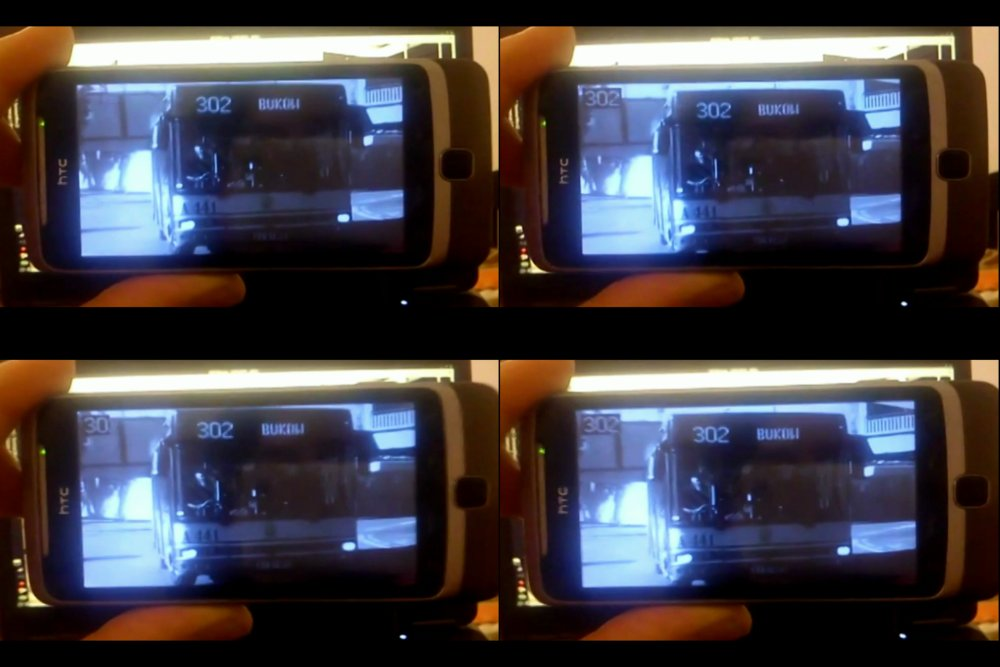
\includegraphics[width=0.9\textwidth]{img/exp_mser_concerns}
    \caption{Wizualizacja testu algorytmu MSER wykonanego przy użyciu telefonu HTC Desire Z}
    \label{fig:mser_example_results}
\end{figure}

Poglądowe rezultaty zostały zaprezentowane na rysunku
\ref{fig:mser_example_results}.
Niestety w~zależności od rozdzielczości zmieniała się podatność
numeru na wykrycie. Dla niewielkich rozdzielczości numer był rozpoznawany
jedynie jako całość, gdzie ograniczeniem geometrycznym wykorzystanym
do tego celu był prostokąt pocztówkowy o~proporcjach 2 na 3 - prezentowany
przykład. Na lewym dolnym obrazie można zaobserwować wykrycie jedynie
pierwszych dwóch cyfr numeru.

W~wyższych rozdzielczościach aby zachować wprowadzone ograniczenie
niezbędne było zastosowanie filtru rozmywającego. Bez filtru
wykrywane regiony reprezentowały poszczególne cyfry składowe numeru.
W~tym przypadku ograniczenie geometryczne wahało się od 1x4 (pionowy
prostokąt) dla jedynki do 2x3 (również prostokąt ustawiony pionowo) dla
pozostałych cyfr.

Zbyt duża liczba czynników wpływających na skuteczność
spowodowała, że pominięto tę metodę w~rozwiązaniu końcowym.
Przykładowe cechy wpływające na decyzję o~zastosowaniu wielu
zestawu parametrów:

\begin{itemize}
    \item krój czcionki: wysokie, wąskie,
    \item inne ograniczenia geometryczne dla zmiennej ilości cyfr
        w~numerze,
    \item stosowanie adaptacyjnych filtrów celem rozmycia obrazów
        w~wyższych rozdzielczościach (autobus bliżej obserwatora),
    \item stosowanie dwóch niezależnych detektorów, oddzielnie dla
        cyfr i~numerów.
\end{itemize}


Pomimo tylu zastrzeżeń jest to druga (po narzędziu Tesseract) metoda, której
wyniki były na tyle obiecujące, że przemyślana implementacja
mogłaby z~powodzeniem zastąpić ostatecznie wykorzystany kaskadowy
detektor oparty na cechach LBP.


\section{Testy narzędzi i~algorytmów wykorzystanych w~rozwiązaniu 
	końcowym}
\label{sec:testynarzedziwykorzystanych}

W podrozdziale tym przedstawione i omówione zostały doświadczenia związane
z~algorytmami, narzędziami i bibliotekami, które wykorzystane zostały
w~ostatecznej wersji programu. Prace, tak jak sam proces wykrywania 
i~odczytywania numeru linii autobusowej podzielone były na trzy etapy:

\begin{enumerate}
	\item Przygotowanie i~przetestowanie detektora frontów autobusów w~scenie.
	\item Przygotowanie i przetestowanie detektora numerów w~wycinku obrazu
	reprezentującym front autobusu.
	\item Przygotowanie i przetestowanie klasyfikatora numerów, reprezentowanych
	przez obrazy o~jednakowych wymiarach.
\end{enumerate}

Wszystkie powyższe kroki wymagały jednego wspólnego elementu - zbiorów obrazów
niezbędnych w~procesie uczenie detektorów i~przygotowywania klasyfikatora.
Ze względu na brak lub nieumiejętność odnalezienia stosownych zbiorów
w~sieci Internet, zbiory obrazów przygotowane zostały własnoręcznie.

Drugim powtarzającym się krokiem dla wszystkich trzech powyższych etapów było
testowanie skuteczności detektorów oraz klasyfikatora przy zmiennych
parametrach zadanych podczas procesu uczenia, detekcji i~klasyfikacji.

Był to jeden z~najbardziej wymagających rozdziałów niniejszej pracy, a~jego
przygotowanie zajęło najwięcej czasu. Wiele wieczorów przeznaczonych zostało 
na oznaczanie i~docinanie kilkunastu tysięcy obrazów. Kolejnym czynnikiem były długie,
nawet kilkudniowe, sesje uczenia detektorów. Na potrzeby sesji testowych,
badających wpływ parametrów wywołania narzędzia uczenia, przygotowano
kilkadziesiąt, jeżeli nie kilkaset detektorów.

Wyniki wielu takich sesji nie zostały zamieszczone na łamach niniejszego opracowania.
Pomimo ogromnych nakładów pracy, czasu i~nerwów, powstrzymano się
od prezentowania bezwartościowych, przekłamanych i~zaburzonych wyników.
Przyczyn było wiele.
Błędne założenia, błędy popełnione podczas przygotowywania zbiorów czy 
przedwczesna optymalizacja (,,źródło wszelkiego zła'') wpłynęły wielokrotnie
na decyzję o~powtórzeniu już raz wykonanego procesu uczenia detektorów.
Poniżej przedstawiono kilka wybranych 
potknięć.

\begin{figure}[h!]
	\centering
	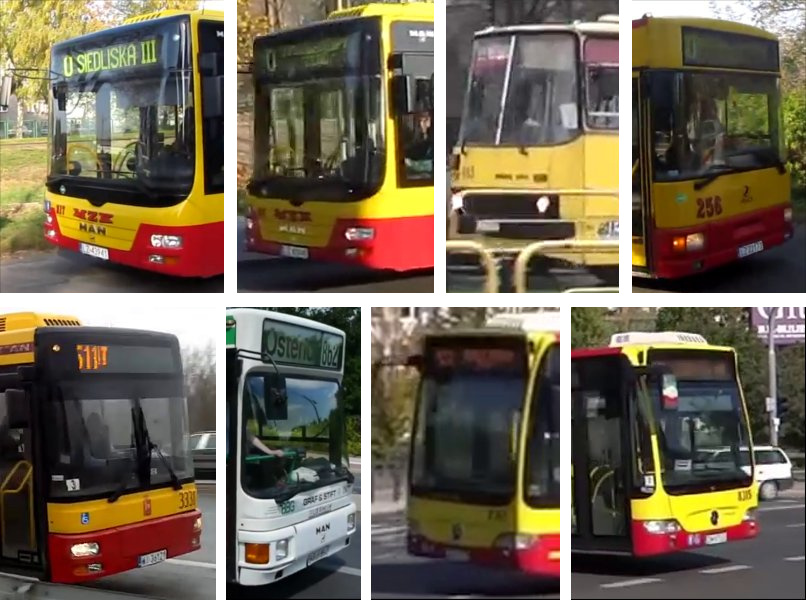
\includegraphics[width=0.6\textwidth]{img/exp_removed_distorted_fronts}
	\caption{Usunięte oznaczenia ze względu na zniekształcenia geometryczne}
	\label{fig:deformation_samples}
\end{figure}

Jeden z~pierwszych błędów popełniony został podczas oznaczania
frontów autobusów. Niestety dopiero testy skuteczności wykazały
istotną wadę przygotowanego zbioru. Wyniki (dużo gorsze od spodziewanych)
automatycznego pomiaru skuteczności poparte organoleptyczną weryfikacją 
typu i~sposobu wykrywania obiektów wykazały błędną klasyfikację próbek pozytywnych
w~zbiorze uczącym. Wszystkie wystąpienia frontu autobusu czołem do fotografującego
oznaczone były jako poprawne i~wartościowe. Po usunięciu zbyt
zniekształconych geometrycznie frontów - jak na rysunku \ref{fig:deformation_samples} -
powtórzony został proces uczenia. Ponownie wykonane zostały też testy skuteczności.

Podczas dalszych prac zbiory uczące i~testowe przygotowywano jeszcze kilkukrotnie.
Raz ze względu
za zbyt mały margines tła pozostawiony wokół szukanego obiektu. Innym powodem 
była forma przechowywanych obrazów. Początkowo przechowywano pełne sceny zawierające wystąpienie
interesującego obiektu, wraz ze współrzędnymi czworokątów okalających.
Takie zbiory z~powodzeniem
nadawały się do wykorzystania podczas testów skuteczności. Kolejne wersje
zbiorów, przechowywano w~postaci wycinków zawierających jedynie interesujące obiekty.
Wymusiło to sporządzenie osobnych zbiorów przechowywanych w~pierwotnej formie, jedynie na potrzeby testów.

\begin{figure}[!h]
	\centering
	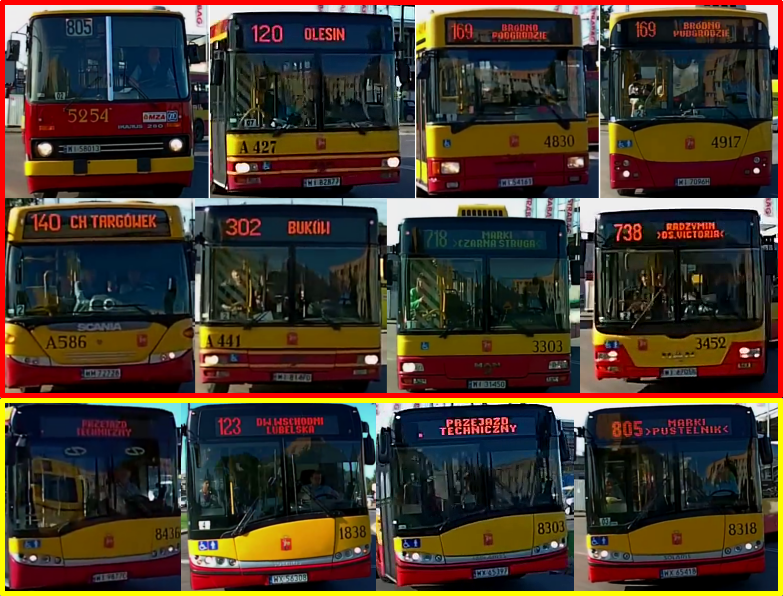
\includegraphics[width=0.6\textwidth]{img/exp_trainig_data_jJ9}
	\caption{Przykładowe elementy jednego ze zbiorów obrazów
		przygotowanych na podstawie
		filmów pobranych z serwisu YouTube}
	\label{fig:jJ9ixBfVR5k_types}
\end{figure}

Kolejny przykład to nieudana próba wykazania różnicy w~skuteczności detektorów
do wyszkolenia których użyto frontów różnych marek i~modeli pojazdów oraz tych
nauczonych przy użyciu takich samych frontów. Podział zilustrowany został na 
rysunku \ref{fig:jJ9ixBfVR5k_types}, gdzie w~czerwonej ramce przedstawione
zostały front typów różnych. Żółta ramka przedstawia próbki jednego typu - 
w~tym przypadku autobusu Solaris Urbino.


Naturalny podział zaobserwowano dopiero podczas półautomatycznego uczenia i~oznaczania
próbek.
Detektory tak przygotowywane faworyzowały
szczególne cechy frontów z~wyświetlaczem. Podczas ostatniego przebiegu
(5000 pozytywnych oznaczeń) zaobserwowano, że detektor
chętnie identyfikuje fronty z~diodowym wyświetlaczem zajmującym 
całą górną część frontu. Przy tak dużej liczbie oznaczeń
cechą szczególną okazał się właśnie ów wyświetlacz. Cecha ta była
na tyle istotna, że oznaczane były również fragmenty boków autobusów
z~wyświetlaczem bocznym, czy fragmenty frontów, na których wyświetlacz
nie zajmował całej długości górnej krawędzi - rysunek
\ref{fig:frontdetectormorph}.

\begin{figure}[!h]
	\centering
	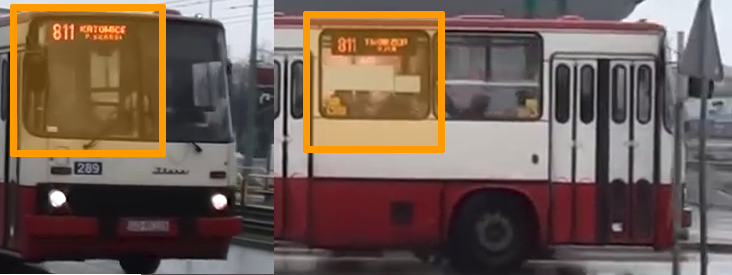
\includegraphics[width=0.95\textwidth]{img/exp_front_detector_curiosity}
	\caption{Tendencja do oznaczania fragmentów z~dużą ilością
		niewielkich elementów w górnej części}
	\label{fig:frontdetectormorph}
\end{figure}

Możliwym rozwinięciem popełnionej implementacji jest więc przeszkolenie
detektora frontowego tak aby wykrywał również tablice boczne. Minusem
tego rozwiązania jest fakt, że z~lokalizowaniem autobusów z~tablicami
drukowanymi detektor radzi sobie znacznie gorzej. Co za tym idzie
zostały one wykluczone z~dalszych rozważań. Aby skutecznie wykrywać
fronty autobusów typu Ikarus lub Jelczy Berliet niezbędny byłby 
dodatkowy dedykowany detektor i~prawdopodobnie dedykowane wersje
pozostałych elementów.

Opisane powyżej problemy, w~dużo mniejszym stopniu powtarzały się w~kolejnych 
dwóch etapach prac. Niektóre błędy możliwe były do wykrycia dopiero po
zestawieniu wszystkich trzech etapów w~jeden proces.

\subsection{Przygotowanie i testy detektora frontów}

W~procesie uczenia wykorzystano zbiór 10145 obrazów reprezentujących fronty autobusów.
Zdjęcia były przygotowane w~ten sposób, że przedstawiały jedynie szukane obiekty
wraz z~niewielką ramką wokół nich. Zachowano oryginalny rozmiar obrazów, których
wymiary mieściły się w~przedziale od 33x33 pikseli do 771x771 pikseli.
Przykładowe elementy zbioru przedstawiono na rysunku \ref{fig:exp_second_crop_sample}.

\begin{figure}[!h]
	\centering
	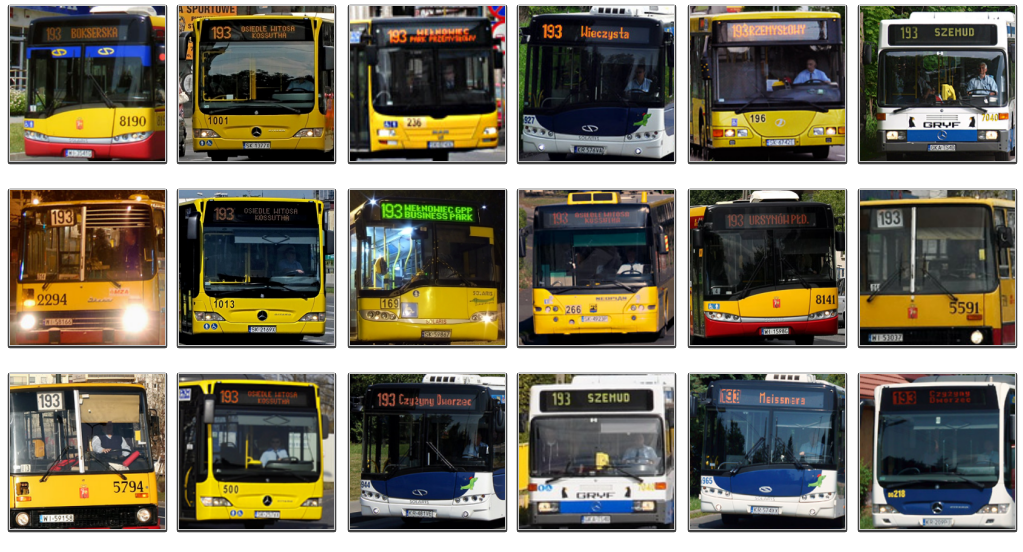
\includegraphics[width=0.8\textwidth]{img/exp_second_crop_sample}
	\caption{Elementy zbioru uczącego - przykład tzw. obrazów pozytywnych}
	\label{fig:exp_second_crop_sample}
\end{figure}

Zbiór z~obrazami tła
przygotowano poprzez wybranie tych klatek z~filmów pobranych z~serwisu
YouTube, które nie
zawierały szukanych obiektów. Fragment zbioru, który w~całości
składał się z~548 elementów, przedstawiono na rysunku \ref{fig:exp_first_background_sample}.

\begin{figure}[!h]
	\centering
	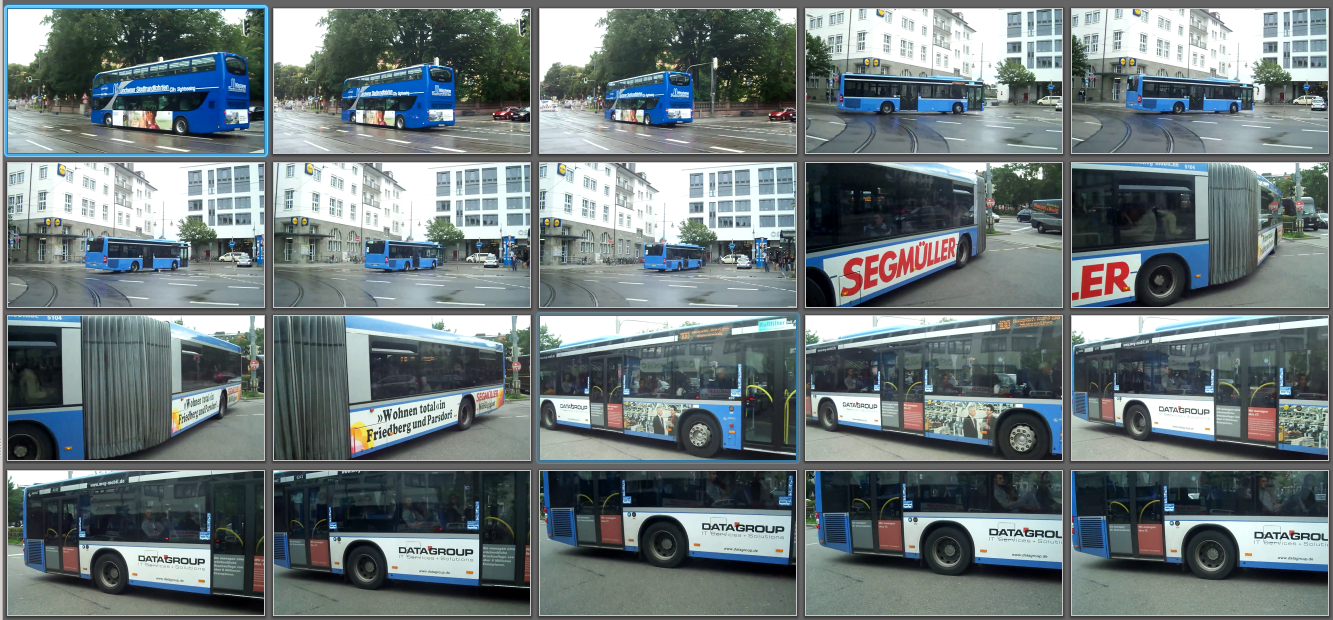
\includegraphics[width=0.9\textwidth]{img/exp_first_background_sample}
	\caption{Przykładowe obrazy tła jednego z 11 zbiorów
		przygotowanych na podstawie
		filmów pobranych z serwisu YouTube}
	\label{fig:exp_first_background_sample}
\end{figure}

Ze względu na brak możliwości wykorzystania zbioru uczącego
w~procesie automatycznych testów skuteczności sporządzono trzeci,
mniejszy zbiór złożony z~pełnych klatek zawierających
fronty autobusów wraz z~ich współrzędnymi. Zbiór ten składał się
z~1954 obrazów. Współrzędne umieszczone były tym razem w~nazwach
plików. Zbiór służył do testowania przygotowanych detektorów. 
Ze względu na zaobserwowaną większą skuteczność detektorów podczas
wykrywania frontów nowego typu (z~tablicą diodową) zbiór testowy
zawierał tylko tego typu obiekty. Fragment przedstawiono na rysunku
\ref{fig:exp_third_whole_sample}. Zbiór uczący wykorzystany do
przygotowywania detektorów zawierał wszystkie typy autobusów.

\begin{figure}[!h]
	\centering
	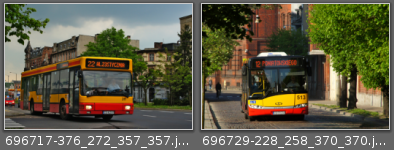
\includegraphics[width=0.6\textwidth]{img/exp_third_whole_sample}
	\caption{Przykładowe obrazy trzeciego zbioru (testowego) 
		wraz ze współrzędnymi widocznymi w nazwach plików}
	\label{fig:exp_third_whole_sample}
\end{figure}

Proporcja ponad 10 tysięcy obrazów pozytywnych do 548 obrazów tła (negatywnych), 
może wydawać się pewnym niedopatrzeniem. Jednak 
w~eksperymentach wykorzystano nieco ponad połowę przygotowanego zbioru. Dodatkowo
sposób działania narzędzia uczącego detektory umożliwiał wielokrotne 
wykorzystanie wielu mniejszych pod-obrazów z~jednego obrazu tła w~dużej
rozdzielczości \ref{fig:exp_false_positive_mechanism}.
 

\begin{figure}[!h]
	\centering
	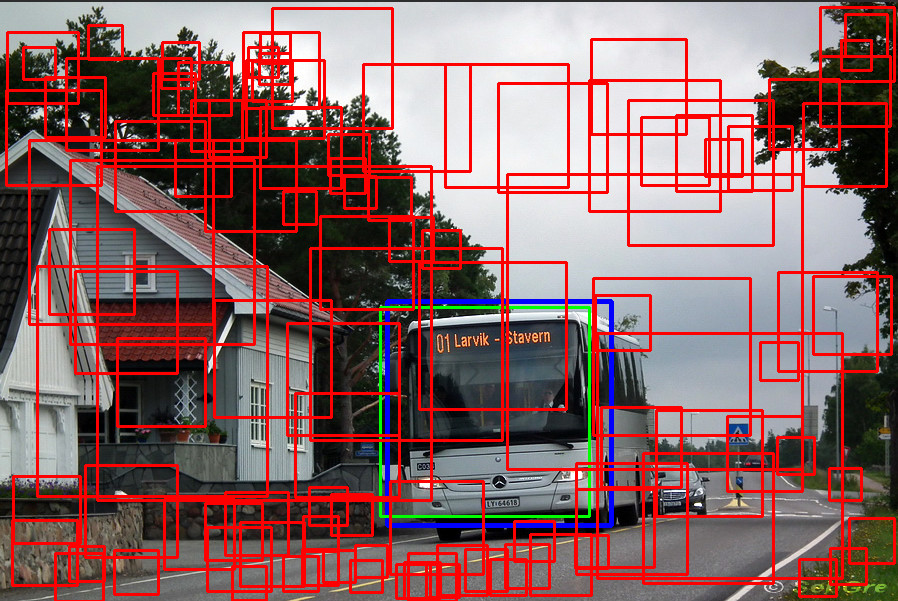
\includegraphics[width=0.6\textwidth]{img/exp_false_positive_mechanism}
	\caption{Sposób wyłuskiwania fałszywych pozytywów z~obrazów tła podczas procesu
		uczenia - analogiczny do liczby błędnych trafień niskiej
		jakości detektora}
	\label{fig:exp_false_positive_mechanism}
\end{figure}

Teoretycznie z~jednej klatki obrazu wyłuskanych mogło być kilkadziesiąt lub
nawet kilkaset pod-obrazów. Czyli analogicznie do sytuacji w~której - jak 
na rysunku 
\ref{fig:exp_false_positive_mechanism}
- bardzo słabej jakości detektor wykrywa dużo fałszywych pozytywów, tak
automat uczący wybiera z~obrazów tła odpowiednie pod-obrazy celem
zmniejszenia liczby
błędnych wykryć uczonego w~ten sposób detektora.

Pierwsze próby związane z~procesem uczenia miały na celu 
wyłonienie parametrów mających największy wpływ na skuteczność 
oraz efektywność trenowanych detektorów.
We wszystkich eksperymentach - jeżeli nie napisane zostało, że
jest inaczej - wykorzystano domyślne parametry wejściowe narzędzia 
\verb|opencv_traincascade|:

\begin{lstlisting}
[-numPos <number_of_positive_samples = 2000>]
[-numNeg <number_of_negative_samples = 1000>]
[-numStages <number_of_stages = 20>]
[-precalcValBufSize <precalculated_vals_buffer_size_in_Mb = 256>]
[-precalcIdxBufSize <precalculated_idxs_buffer_size_in_Mb = 256>]
[-featureType <{HAAR(default), LBP, HOG}>]
[-w <sampleWidth = 24>]
[-h <sampleHeight = 24>]
[-bt <{DAB, RAB, LB, GAB(default)}>]
[-minHitRate <min_hit_rate> = 0.995>]
[-maxFalseAlarmRate <max_false_alarm_rate = 0.5>]
[-weightTrimRate <weight_trim_rate = 0.95>]
[-maxDepth <max_depth_of_weak_tree = 1>]
[-maxWeakCount <max_weak_tree_count = 100>]
\end{lstlisting}

Pierwsza iteracja uczenia detektorów miała na celu przetestowanie
parametrów, jakie można zadać narzędziu uczącemu \verb|opencv_traincascade|.
Na początku
uczono detektory oparte na
cechach LBP. Zgodnie z dokumentacją \cite{OCV:cascadeclassifiertraining}, ze względu na wykorzystanie liczb całkowitych,
metoda ta (w porównaniu do klasycznego detektora opartego na cechach HAAR-a) powinna być
kilkukrotnie szybsza zarówno podczas uczenia jak i wykrywania obiektów.

Pierwszy test miał wskazać optymalny stosunek wykorzystania próbek pozytywnych
do negatywnych. W~tabeli 4.4 przedstawiono wyniki dla detektora LBP, 
złożonego z 10 kaskad
przy liczbie 5000 próbek pozytywnych i zmiennej liczbie obrazów tła.

\begin{table}[!h]
	\centering                                                          
	\caption{Skuteczność detektorów wyszkolonych 
		dla różnych wartości parametrów narzędzia traincascade 
		- zmienna liczba próbek negatywnych dla 5000 pozytywów.
	}
	\begin{tabular}{r|c|c|c|l}
		Liczba próbek & Poprawne & Błędne   & Czas         & Czas    \\
		negatywnych   & wykrycia & pozytywy & wykrycia (sek) & uczenia (min) \\
		\hline
		2000        & 593      & 211002   & 1,098       & 11 \\
		3000        & 594      & 195190   & 0,989       & 12,5 \\
		4000        & 1110     & 145873   & 0,911       & 15 \\
		5000        & 840      & 169297   & 0,964       & 16,5 \\
		6000        & 876      & 161671   & 0,917       & 18 \\
		7000        & 1580     & 98354    & 0,823       & 22 \\
		8000        & 1486     & 104533   & 0,781       & 25 \\
		9000        & 1641     & 76363    & 0,776       & 33,5 \\
		10000       & 1661     & 77879    & 0,741       & 40 \\
	\end{tabular} 
	\label{tab:it1detectorlist}
\end{table}

Mając do dyspozycji 1903 obrazy z oznaczonymi frontami, przetestowano 80 detektorów
wyszkolonych przy zmiennej liczbie obrazów tła. Wyniki zamieszczone w powyższej tabeli
\ref{tab:it1detectorlist} wskazują kilka ciekawych zależności. Po pierwsze przy stosunku próbek negatywnych do
pozytywnych równym 1:1 skuteczność była nie tylko niezadowalająca, lecz wysoce niestabilna.
Osiągano skrajnie różne wyniki dla niewielkich 
różnic w~liczbie próbek negatywnych:

\begin{itemize}
	\item 3800 - 256/1903 (skuteczność 13\%),
	\item 4000 - 1110/1903 (skuteczność 58\%).
\end{itemize}

\begin{figure}[h!]
	\begin{center}
		\begin{tikzpicture}
		\begin{axis}[
		xlabel={$Liczba\ probek\ negatywnych$},
		minor y tick num=1,
		legend style={at={(0.55,0.90)},anchor=north west},
		width=\textwidth*0.9, height=6cm, ymajorgrids, xmajorgrids
		]
		\addplot [only marks, color=blue] table {data/front_pos_5000_neg_2000_1000_effectiveness.dat};
		\addlegendentry{skuteczność (\%)}
		\addplot [only marks, color=red] table {data/front_pos_5000_neg_2000_1000_false_positives.dat};
		\addlegendentry{liczba błędów (w tysiącach)}
		\end{axis}
		\end{tikzpicture}
	\end{center}
	\caption{Skuteczność w procentach oraz liczba błędnych trafień
		w~zależności od liczby próbek negatywnych wykorzystanych 
		w~procesie uczenia.}
	\label{chart:5000to2000_10000neg}
\end{figure}

W~omawianym eksperymencie przygotowano 80 detektorów, co może wydawać
się lekką przesadą. Przeprowadzono go jednak i~opisano w~celu nakreślenia
problemu jaki pojawia się przy zagadnieniach związanych
z~uczeniem maszynowym
w~kontekście wykrywania obiektów. Mowa o~efekcie skali 
i~ogromnych zbiorach obrazów niezbędnych do przygotowania
detektorów i~klasyfikatorów o~dobrych parametrach. 
Jak to zostało podkreślone, przy niewielkiej liczbie próbek - na poziomie kilku tysięcy 
(3800 - 4000) - pojawienie się kliku(set)
specyficznych obrazów może
zupełnie zmienić charakterystykę uczonego detektora. Wraz ze wzrostem liczebności zbioru
obrazów tła skuteczność szkolonych detektorów stabilizowała się na poziome 1600[+/-50]/1903
(84[+/-3]\%).

Oczywistym wręcz wnioskiem jest to, że większa liczba negatywnych
próbek wykorzystana w~procesie uczenia daje w~rezultacie detektor 
o~lepszych parametrach.
Co ciekawe, wraz ze wzrostem liczby obrazów tła, odnotowano nie tylko spadek 
wykryć błędnych lecz
co ważniejsze, znaczny wzrost skuteczności uczonych detektorów. Wartości te były ze sobą
skorelowane - ,,lepsze'' detektory miały większą skuteczność przy jednoczesnym mniejszym
odsetku błędnych trafień - wykres \ref{chart:5000to2000_10000neg}. Pierwsza
wersja detektora była podatna na pomyłki - czerwone kropki na wykresie 
symbolizują setki tysięcy błędnych oznaczeń.

Rosnąca liczba wykorzystanych obrazów tła, oprócz poprawienia skuteczności, miała
też wpływ na wydajność, czyli szybkość wykrywania obiektu w~obrazie. Najprawdopodobniej
fragmenty obrazów nie zawierające frontu autobusu były częściej i~szybciej odrzucane jako
niepoprawne, przy jednoczesnym wykorzystaniu mniejszej liczby cech oraz kaskad.
Wraz ze wzrostem liczby negatywnych próbek wykorzystanych w~procesie przygotowywania
detektora, z~dwóch do dziesięciu tysięcy uzyskano wzrost wydajności rzędu 300 milisekund - 
tabela \ref{tab:it1detectorlist} (test wykonany na maszynie z~procesorem AMD Sempron 2800+).

Kolejnym testowanym elementem była ogólna liczba pozytywnych i negatywnych próbek
wykorzystanych w procesie uczenia. Wyniki przeprowadzonego testu przedstawiono 
na wykresie \ref{chart:500to11200pos_2x_neg}.

\begin{figure}[h!]
	\begin{center}
		\begin{tikzpicture}
		\begin{axis}[
		xlabel={$Liczba\ probek\ pozytywnych$},
		minor y tick num=1,
		legend style={at={(0.55,0.90)},anchor=north west},
		width=\textwidth*0.9, height=12cm, ymajorgrids, xmajorgrids
		]
		\addplot [only marks, color=blue] table {data/front_pos_500_10000_effectiveness.dat};
		\addlegendentry{skuteczność (\%)}
		\addplot [only marks, color=red] table {data/front_pos_500_10000_false_positives.dat};
		\addlegendentry{liczba błędów (w tysiącach)}
		\node[anchor=west] (source) at (axis cs:1700,190){Skuteczność równa 90\%};
		\node (destination) at (axis cs:2200,95){};
		\draw[->](source)--(destination);
		\end{axis}
		\end{tikzpicture}
	\end{center}
	\caption{Skuteczność w procentach oraz liczba błędnych trafień
		w~zależności od liczby próbek pozytywnych (i negatywnych - dwukrotność 
		liczby próbek pozytywnych) wykorzystanych 
		w~procesie uczenia.}
	\label{chart:500to11200pos_2x_neg}
\end{figure}

Pierwszą ciekawą sytuacją na wykresie \ref{chart:500to11200pos_2x_neg} są wartości
osiągnięte dla 2200 próbek pozytywnych (4400 negatywów). Skuteczność detektora
jest wtedy po raz pierwszy równa 90\%. Po raz pierwszy liczba błędów jest też mniejsza
od 90 tys. - na wykresie pierwsza niebieska kropka nad kropką czerwoną. 
Sytuacja ta powtórzyła się
jeszcze 13 razy, przy czym przedostatnia para - skuteczność 82\% i~95 tys. błędnych trafień - 
pokazuje jak ważna jest dostatecznie duża liczba elementów w~zbiorach
wykorzystanych podczas przygotowywania detektorów. Zmiana liczby próbek o~100
powoduje różnicę w~skuteczności rzędu kilku procent.

Teoretycznie, w~dalszych
eksperymentach można by wykorzystywać wartość 2200 próbek pozytywnych (4400 negatywów).
Detektor tak przygotowany wykrył tylko 28 mniej frontów (na 1903 oznaczonych frontów 
testowych), przy o~ponad 10 tys. większej liczbie błędów od detektora do przygotowania
którego wykorzystano 3000 więcej obrazów reprezentujących front oraz 6000 więcej próbek negatywnych. Nie oznacza to bynajmniej, że detektory te mają podobne charakterystyki.
Wyniki tu zaprezentowane zależą znacznie od przygotowanego zbioru testowego, złożonego
z~pełnych klatek reprezentujących oznaczone 1903 wystąpienia frontów autobusów z~wyświetlaczem
ledowym. Niewielka liczba elementów zbioru pozwala jedynie na zaobserwowanie trendu, 
kiedy to większa liczba elementów w~zbiorach uczących przekłada się na detektory o~lepszych
parametrach. Niemożliwe jest wyłonienie konkretnych wartości do przygotowania detektora
o~najlepszych parametrach - największej skuteczności i~najmniejszej podatności na pomyłki.
W~dalszych eksperymentach wykorzystano liczbę próbek pozytywnych na poziomie 5000.
Pozostawiono stosunek (1 do 2) próbek pozytywnych do negatywnych ustanowiony na podstawie wyników poprzedniego eksperymentu. Co za tym idzie, wykorzystano 10 tys. próbek tła.

\begin{table}[!h]
	\centering                                                          
	\caption{Liczba poprawnie wykrytych frontów, liczba błędów oraz czasy uczenia 
		i detekcji w zależności od ilości kaskad wykorzystanych w procesie uczenia 
		detektorów.}
	\begin{tabular}{r|r|r|c|l}
		Liczby    & Poprawne     & Błędy  & Średni czas    & Czas     \\
		kaskad    & wykrycia     &        & wykrycia (sek) & uczenia  \\
		\hline
		20        & 1801 (95\%)  & 148    & 0.737   & 87 godz.\\
		19        & 1818 (96\%)  & 219    & 0.738   & 42 godz.\\
		18        & 1834 (96\%)  & 389    & 0.735   & 21 godz.\\
		17        & 1854 (97\%)  & 835    & 0.732   & 12 godz.\\
		16        & 1865 (98\%)  & 1736   & 0.730   & 7 godz. \\
		15        & 1879 (99\%)  & 3495   & 0.738   & 4 godz. \\
		14        & 1880 (99\%)  & 6683   & 0.729   & 2 godz. \\
		13        & 1887 (99\%)  & 12940  & 0.762   & 2 godz. \\
		12        & 1871 (98\%)  & 24859  & 0.734   & 1 godz. \\
		11        & 1822 (96\%)  & 45749  & 0.747   & 55 min. \\
		10        & 1661 (87\%)  & 77879  & 0.742   & 2 godz. \\
		9         & 1258 (66\%)  & 128532 & 0.764   & 33 min. \\
		8         & 525  (27\%)  & 201264 & 0.891   & 27 min. \\
		7         & 122  (6.4\%) & 299567 & 1.636   & 23 min. \\
		6         & 7    (0.4\%) & 508466 & 6.219   & 19 min. \\
		5         & 0    (0.0\%) & 858169 & 12.30   & 15 min. \\
	\end{tabular} 
	\label{tab:cascade_2_effi}
\end{table}

Oba dotychczasowe doświadczenia były wykonane dla stałej - równej 10 - liczby kaskad.
Następny test miał na celu przetestowanie wpływu tego parametru na właściwości
przygotowywanego detektora. Tak jak to zostało wspomniane wykorzystano 5000 oznaczonych 
wystąpień frontów oraz
10000 próbek negatywnych. Był to ostatni test wykonany na starej konfiguracji sprzętowej
opartej na procesorze AMD Sempron 2800+. Celem testu było zbadanie wpływu liczby kaskad
na skuteczność i~wydajność uczonych detektorów. Wyniki zaprezentowane zostały w tabeli 
\ref{tab:cascade_2_effi}.


W~dalszych eksperymentach wykorzystano domyślną wartość - 20 kaskad. Ze względu
na liczbę poprawnie wykrytych frontów nie jest to co prawda optymalny wybór,
jednak skuteczność na poziomie 95\% jest wystarczająco dobra jako punkt startowy. Dodatkowo
specyfika programu końcowego, czyli ciągłe pobieranie klatek zawierających
nadjeżdżający autobus wymaga jak najmniejszej liczby błędnych trafień przy 
dostatecznym tylko odsetku poprawnych wykryć, który nie musi być za bardzo wyśrubowany.
Zgodnie z rysunkiem \ref{fig:dist2res}
numer linii jest widoczny i możliwy do odczytania, gdy front autobusu znajduje 
się w~odległości
między 30 a~40 metrów od obserwatora. Zakładając, że prędkość autobusu wjeżdżającego
do zatoki będzie wynosić 30 km/h do pełnego zatrzymania jest jakieś 4-6 sekund. 
Podczas jednej
takiej sesji, dysponując prędkością rejestracji na poziomie 20 klatek na sekundę, 
pobranych
zostanie 100(+/-20) klatek. W~takim przypadku skuteczność nawet na poziomie 50\% 
umożliwia pobranie około 50 wycinków reprezentujących front autobusu. 
Skuteczność na poziomie
95\% jest zatem więcej niż zadowalająca. Minusem był w~tym przypadku czas potrzebny
na wyszkolenie detektora. W~dalszych eksperymentach podczas optymalizacji wyszukiwania
frontu autobusu w~scenie używano detektora przygotowanego z~wykorzystaniem następujących 
parametrów:

\begin{lstlisting}[caption={Ostateczne parametry wywołania narzędzia opencv\_traincascade},label=lst:front_end_parameter_values]
[-numPos 5000]
[-numNeg 10000]
[-numStages 20] //__________________________________ wartosc domyslna
[-precalcValBufSize <precalculated_vals_buffer_size_in_Mb = 256>]
[-precalcIdxBufSize <precalculated_idxs_buffer_size_in_Mb = 256>]
[-featureType LBP]
[-w 30]
[-h 30]
[-bt <{DAB, RAB, LB, GAB(default)}>] //_____________ wartosc domyslna
[-minHitRate 0.995] //______________________________ wartosc domyslna
[-maxFalseAlarmRate 0.5] //_________________________ wartosc domyslna
[-weightTrimRate 0.95] //___________________________ wartosc domyslna
[-maxDepth <max_depth_of_weak_tree = 1>] //_________ wartosc domyslna
[-maxWeakCount <max_weak_tree_count = 100>] //______ wartosc domyslna
\end{lstlisting}

Powyższy proces uczenia jako ostatni został przeprowadzony z~wykorzystaniem
starej konfiguracji sprzętowej, opartej na procesorze AMD Sempron 2800+ i~trwał
3~dni i~15~godzin. Wszystkie kolejne eksperymenty wykonywane były na jednostce
wyposażonej w~procesor Intel Core i5-3570K. Aby zaprezentować różnicę
w~wydajności obu maszyn, przygotowano detektor dla takich samych parametrów
wejściowych jak w~ostatnim doświadczeniu. Wartości końcowe przedstawione zostały
w~tabeli \ref{tab:cpu_comparison}.

\begin{table}[!h]
	\centering                                                          
	\caption{Zestawienie czasów wykonania i~przygotowania detektorów,
		w~zależności od modelu procesora}
	\begin{tabular}{c|c|c}
		Procesor  & Średni czas      & Czas     \\
		& wykrycia (w sek) & uczenia  \\
		\hline
		Sempron 2800+        & 0.737  & 87 godz. \\
		Core i5 3570K        & 0.186  & 24 godz. \\
	\end{tabular} 
	\label{tab:lbp_hog_haar}
\end{table}

Osiągnięto czterokrotnie krótszy czas wykrywania frontu w~scenie i~niemal 
czterokrotnie krótszy czas potrzebny na przygotowanie detektora. Na starym 
sprzęcie czas uczenia wynosił 3 dni i 15 godzin, podczas gdy nowa maszyna
poradziła sobie z~tym zadaniem w~dokładnie jeden dzień. Wykorzystując nowszy
sprzęt wykonao ostatni test parametrów wywołania. Przygotowano trzy detektory
oparte na cechach LBP, HOG oraz HAAR. Pozostałe parametry ustawione zostały
zgodnie z~ostatnim testem, jak na wydruku \ref{lst:front_end_parameter_values}.
Wyniki dla trzech przebiegów zamieszczono w tabeli \ref{tab:cpu_comparison}.

\begin{table}[!h]
	\centering                                                          
	\caption{Liczba poprawnie wykrytych frontów, liczba błędów oraz czasy uczenia 
		i detekcji w zależności od typu cech wykorzystanych w procesie uczenia 
		detektorów.}
	\begin{tabular}{r|r|r|c|l}
		Typ    & Poprawne     & Błędy  & Średni czas    & Czas     \\
		cech   & wykrycia     &        & wykrycia (sek) & uczenia  \\
		\hline
		LBP        & 1801 (95\%)  & 148    & 0.184   & 24 godz.\\
		HOG        & 1398 (73\%)  & 964    & 0.133   & 19 godz.\\
		HAAR       & 1860 (98\%)  & 185    & 0.165   & 100 godz.\\
	\end{tabular} 
	\label{tab:cpu_comparison}
\end{table}

Głównym celem była weryfikacja detektora przygotowanego z~wykorzystaniem
cech typu HAAR: zarówno czasu potrzebnego do jego wyszkolenia, jak i~skuteczności
oraz co najważniejsze wydajności przy wykrywaniu obiektów - średniego czasu 
wykrycia pojedynczego obiektu w~scenie - na podstawie 1903 próbek testowych.

Zaskoczeniem jest słaby wynik detektorów opartych na cechach HOG. Nie dziwi doskonały
wynik detektora HAAR-a, jednak ponad czterokrotnie dłuższy czas uczenia i~większa 
liczba błędów niwelują jego główną zaletę, jaką jest skuteczność na poziomie 98\%.
Inny od oczekiwanych jest też wynik pomiaru wydajności podczas detekcji obiektów
w~scenie. Spodziewano się, że czas uczenia potrzebny na przygotowanie detektora
będzie skorelowany z~czasem detekcji pojedynczego frontu w~obrazie.
Tymczasem wydajność wszystkich detektorów jest zbliżona, a~co 
gorsza HAAR jest w~tej dziedzinie szybszy od LBP
(wynik drugiego przebiegu testowego [w kontekście szybkości wykrywania] 
uruchomionego na maszynie
z procesorem Intel Core i7-4710MQ dla cech LBP, HOG i HAAR to odpowiednio: 0.190, 
0.136, 0.158). Sytuacja może niestety wyglądać zgoła inaczej na urządzeniu
mobilnym. Trudno bowiem oprzeć się wrażeniu, że w~eksperymencie tym
sprawdzana była nie tylko implementacja algorytmów lecz co gorsza 
wydajność konkretnego procesora w~dziedzinie obliczeń na liczbach całkowitych
(LBP) oraz zmiennoprzecinkowych (HAAR). Wyniki jednak mówią same za
siebie i~trudno z~nimi polemizować.

\subsubsection{Testy wykonane podczas wywołania detektora}

W~celu zmniejszenia złożoności obliczeniowej przeprowadzone zostały
testy na zmniejszonych klatkach wejściowych. 
Wykonano szereg pomiarów skuteczności dla zmiennej
wysokości obrazów, przy zachowaniu ich proporcji. Poglądowe wyniki zaprezentowano na
wykresie \ref{chart:img_height2hitratio}, gdzie niebieskie kropki oznaczają skuteczność w~procentach, a czerwone liczbę
błędnie oznaczonych obszarów, które nie przedstawiają szukanych obiektów.

\begin{figure}[h!]
	\begin{center}
		\begin{tikzpicture}
		\begin{axis}[
		xlabel={$Wysokosc\ obrazu$},
		minor y tick num=1,
		legend style={at={(0.72,0.32)},anchor=north west},
		width=\textwidth*1, height=12cm, ymajorgrids, xmajorgrids
		]
		\addplot [only marks, color=blue] table {data/front2hitra.dat};
		\addlegendentry{skuteczność [\%]}
		\addplot [only marks, color=red] table {data/front2false.dat};
		\addlegendentry{liczba błędów}
		\addplot [only marks, color=green] table {data/front2effi.dat};
		\addlegendentry{wydajność [ms]}
		\end{axis}
		\end{tikzpicture}
	\end{center}
	\caption{Skuteczność w procentach, liczba błędnych trafień oraz
		wydajność detektorów - w milisekundach na klatkę obrazu -
		w~zależności od wysokości obrazu wejściowego}
	\label{chart:img_height2hitratio}
\end{figure}

Ostatecznie wysokość obrazu ustawiono na 300 pikseli. Była to najmniejsza - jedna
z~trzech - wartość dla której skuteczność podskoczyła do 97\%.
Detektor posiadał wtedy:
\begin{itemize}
	\item zwiększoną skuteczność do poziomu 97\% (1840/1903),
	\item zmniejszoną tendencję do błędów - odnotowano 56 niepoprawnych oznaczeń,
	\item zmniejszony czas potrzebny do wykrycia frontu w~scenie 
	ze~190 do 40 milisekund.
\end{itemize}

Podsumowując, dzięki przeskalowaniu obrazu wejściowego do z~góry zadanych
300 pikseli poprawiono wszystkie parametry detektora. 
Głównym celem było zwiększenie wydajności projektowanego narzędzia, przy
okazji w~zupełnie nieoczekiwany sposób poprawie uległy pozostałe dwa parametry
pierwszego z~wykorzystanych podzespołów rozwiązania docelowego.
W~kolejnych podrozdziałach opisane zostały podobne zestawy kroków
poczynione w~celu przygotowania pozostałych dwóch podzespołów:

\begin{itemize}
	\item detektora numerów w~zlokalizowanym froncie autobusu,
	\item czytnika numeru z~fragmentu obrazu reprezentującego numer linii autobusowej.
\end{itemize}

\subsection{Detektor numerów}

Podobnie jak podczas przygotowywania detektora frontów,
tak w~trakcie prac nad detektorem numerów pojawiły się pewne problemy.
Do wyszkolenia jednej z~pierwszych wersji
detektora użyto 450 oznaczonych wystąpień numerów (jedno, dwu
i~trzycyfrowych) oraz 800 instancji tła. Ze względu na problemy podczas
szkolenia detektora dla większej liczby pozytywnych i~negatywnych 
instancji zaprzestano zwiększania ich ilości i~przez dłuższy czas
była to ,,najlepsza'' i~jedyna wersja detektora. Problem polegał na
zawieszeniu się procesu uczenia na jednym z~etapów i~gdy normalnie 
cała procedura liczona była w~dziesiątkach minut (maksymalnie 1-2 godziny)
to dla zbyt dużej liczby - w~szczególności obrazów tła - proces potrafił
utknąć na danym etap na dobę. Późniejsze testy wykazały, że
problem dotyczył jedynie implementacji na środowisku Windows. 
Narzędzia skompilowane i~uruchomione na systemie Linux nie 
wykazywały tendencji do zawieszania się. Była to jedna z~wielu 
niedogodności napotkanej po drodze do implementacji końcowej. 
Przy procesach trwających nawet do kilku dni, wszystkie nieudane próby
były co najmniej deprymujące i~sukcesywnie wpływały na decyzję
o~ograniczaniu ilości wykonywanych eksperymentów.


\begin{table}[!h]
	\centering                                                          
	\caption{Liczba poprawnie wykrytych frontów, liczba błędów oraz czasy uczenia 
		i detekcji w zależności od liczby próbek negatywnych wykorzystanych w procesie uczenia 
		detektorów.}
	\begin{tabular}{r|r|r|c|l}
		Liczba ob-& Poprawne     & Błędy  & Średni czas    & Czas uczenia    \\
		razów tła& wykrycia     &        & wykrycia (ms) & (godz.)  \\
		\hline
		
		2000 &	2662 (86\%) &	741 &	18 & 2 \\
		2500 &	2542 (82\%) &	454 &	16 & 4 \\
		3000 &	2466 (80\%) &	264 &	15 & 19 \\
		3500 &	2458 (79\%) &	308 &	15 & 12 \\
		4000 &	2452 (79\%) &	264 &	16 & 19 \\
		4500 &	2529 (82\%) &	310 &	15 & 35 \\
		5000 &	2436 (79\%) &	278 &	15 & 57 \\
	\end{tabular} 
	\label{tab:2000pos4negFunction}
\end{table}

Jako pierwszy, przeprowadzono eksperyment mający na celu wyłonienie
odpowiedniego stosunku próbek pozytywnych do negatywnych.
W~przypadku detektorów frontów autobusów wykorzystano stosunek 1:2. W~tym eksperymencie w~procesie przygotowywania
detektorów wykorzystano 2000 pozytywnych i~zmienną liczbę próbek
negatywnych.
Wyniki eksperymentu zamieszczone w~tabeli \ref{tab:2000pos4negFunction}
wykazują, że wpływ liczby próbek negatywnych na charakterystykę
przygotowywanych detektorów zatrzymuje się na poziomie 2:3. 
Dla wartości 3000 obrazów tła odnotowano ostatni wpis z~tendencji spadkowej
w~kontekście liczby błędnych trafień. W~kolejnych wierszach
można zaobserwować oscylację wokół liczby 275(+/-30).

Biorąc pod uwagę powyższe wyniki ostateczny detektor numeru wykonano
dla 6 tys. próbek pozytywnych i 10 tys. obrazów tła. Okno przesuwne
miało 30 pikseli wysokości i~40 szerokości. Tak przygotowany
detektor osiągnął skuteczność na poziomie 90\% (2796/3100). Liczba fragmentów
obrazów błędnie zaklasyfikowana jako numer była równa 283.

\subsubsection{Testy wykonane podczas wywołania detektora}

Podobnie jak w~poprzednim przypadku, tak tutaj wykonano eksperyment
ze~skalowaniem obrazów wejściowych reprezentujących front autobusu.
Wyniki pomiarów skuteczności dla zmiennej wysokości i~szerokości
obrazów zaprezentowano na wykresie \ref{chart:front_height2hitratio}.

\begin{figure}[h!]
	\begin{center}
		\begin{tikzpicture}
		\begin{axis}[
		ylabel={$Trafienia$},
		xlabel={$Wysokosc\ obrazu$},
		minor y tick num=1,
		legend style={at={(0.04,0.94)},anchor=north west},
		width=\textwidth*0.6, height=6cm
		]
		\addplot [only marks, color=blue] table {data/num/front2hitra.dat};
		\addlegendentry{skuteczność}
		\addplot [only marks, color=red] table {data/num/front2false.dat};
		\addlegendentry{liczba błędów}
		\end{axis}
		\end{tikzpicture}
	\end{center}
	\caption{Skuteczność w procentach oraz liczba błędnych trafień 
		w~zależności od wysokości obrazu wejściowego}
	\label{chart:front_height2hitratio}
\end{figure}

W~dalszych testach wykorzystano wysokość na poziomie 250 pikseli. 
Dla tej wartości po raz pierwszy osiągnięto skuteczność równą 93\% (2891/3100).
Co ważne, nieznacznie zmniejszyła się liczba błędów (z 283 do 250). 
Czas potrzebny na przeskanowanie jednej klatki obrazu
zmniejszył się z~18 do 13 milisekund.

Następnym krokiem, pominiętym w~procesie przygotowywania poprzedniego
detektora, było zbadanie wpływu współczynnika skalowania okna przesuwnego
na skuteczność i~wydajność detektora. Wyniki pomiarów zaprezentowane
zostały na wykresie \ref{chart:scale_factor2hitratio}.

\begin{figure}[h!]
	\centering
	\begin{subfigure}{.49\linewidth}\centering
		\begin{tikzpicture}
		\begin{axis}[
		width=\linewidth,   %%<-------- here
		ylabel={$Trafienia$},
		xlabel={$Wspolczynnik\ skalujacy$},
		minor y tick num=1,
		legend style={at={(0.54,0.94)},anchor=north west},
		height=6cm
		]
		\addplot [only marks, color=blue] table {data/num/scalefactor/front2hitra.dat};
		\addlegendentry{skuteczność}
		\end{axis}
		\end{tikzpicture}
	\end{subfigure}
	\hfill
	\begin{subfigure}{.49\linewidth}\centering
			\begin{tikzpicture}
			\begin{axis}[
			width=\linewidth,   %%<-------- here
			ylabel={$Bledy$},
			xlabel={$Wspolczynnik\ skalujacy$},
			minor y tick num=1,
			legend style={at={(0.48,0.94)},anchor=north west},
			height=6cm
			]
			\addplot [only marks, color=red] table {data/num/scalefactor/front2false.dat};
			\addlegendentry{liczba błędów}
			\end{axis}
			\end{tikzpicture}
	\end{subfigure}
	\caption{Skuteczność w procentach oraz liczba błędnych trafień 
		w~zależności od współczynnika skalowania okna przesównego}
	\label{chart:scale_factor2hitratio}
\end{figure}

Współczynnik skalowania ustawiony został na 1.05. Dla tej wartości
detektor posiadał znacznie lepszą skuteczność równą 95\%. Problemem była 
zwiększona liczba błędów (423) oraz dłuższy czas wyszukiwania frontu w~scenie, 
który wydłużył się z~13 do 22 milisekund.

Kolejnym krokiem była minimalizacja liczby niepoprawnych wykryć, którą
próbowano osiągnąć poprzez wprowadzenie szeregu ograniczeń geometrycznych. 
Na tym etapie nie próbowano wprowadzać optymalizacji. Wszystkie 
pomiary czasów były zbierane na potrzeby późniejszych eksperymentów
gdyby okazało się, że złożoność obliczeniowa nie pozwala na skuteczne
działanie programu na telefonie.
Jako pierwszy wykonano test ze~zmiennym maksymalnym rozmiarem 
okna przesuwnego. Wyniki eksperymentu przedstawiono na wykresie
\ref{chart:front_max2ratio}.

\begin{figure}[h!]\centering
	\begin{subfigure}{.49\linewidth}\centering
		\begin{tikzpicture}
		\begin{axis}[
		ylabel={$Trafienia$},
		xlabel={$Maksymalne\ wymiary\ okna$},
		minor y tick num=1,
		legend style={at={(0.54,0.22)},anchor=north west},
		width=\linewidth, height=6cm
		]
		\addplot [only marks, color=blue] table {data/num/max/front2hitra.dat};
		\addlegendentry{skuteczność}
		\end{axis}
		\end{tikzpicture}
	\end{subfigure}	
	\hfill
	\begin{subfigure}{.49\linewidth}\centering
		\begin{tikzpicture}
		\begin{axis}[
		width=\linewidth,   %%<-------- here
		ylabel={$Bledy$},
		xlabel={$Wspolczynnik\ skalujacy$},
		minor y tick num=1,
		legend style={at={(0.48,0.22)},anchor=north west},
		height=6cm
		]
		\addplot [only marks, color=red] table {data/num/max/front2false.dat};
		\addlegendentry{liczba błędów}
		\end{axis}
		\end{tikzpicture}
	\end{subfigure}
	\caption{Skuteczność w procentach oraz liczba błędnych trafień 
		w~zależności od maksymalnych wymiarów okna przesuwnego}
	\label{chart:front_max2ratio}
\end{figure}

Maksymalne wymiary okna ustawiono na 55x55 pikseli\footnote{Okno nie było
	kwadratowe. Uproszczenie zastosowane w~kodzie aplikacji ograniczało dłuższą krawędź
	okna. Czyli przy stosunku 3:2 maksymalne wymiary okna wynosiły 55x36}. Skuteczność detekcji pozostała
bez zmian. Zmniejszyła się natomiast liczba błędów - z~423 do 330. Poprawie
uległa też wydajność. 
Na tym etapie czas potrzebny na przeszukanie jednego wycinka obrazu
reprezentującego front autobusu wynosił średnio 10 milisekund.

Ostatnim ze sposobów na ograniczenie błędnych trafień było zawężenie
obszaru poszukiwań do lewego górnego rogu obrazu reprezentującego
front autobusu. Na poglądowym rysunku nr \ref{fig:frontupperleft} przedstawiono
przykładowy dobór parametrów - czyli jak duży powinien być ów ,,lewy górny róg''.

\begin{figure}[!h]
    \centering
    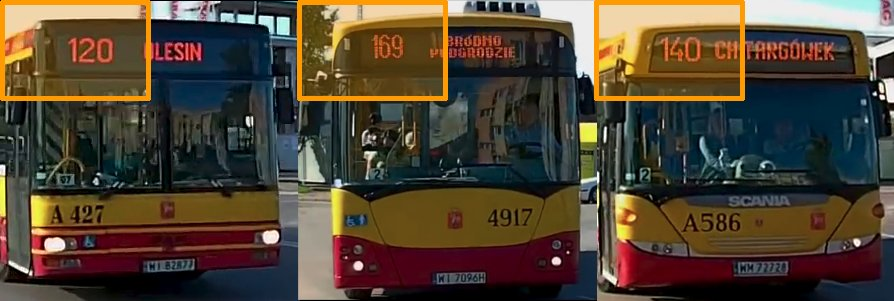
\includegraphics[width=0.95\textwidth]{img/exp_front_upper_left}
    \caption{Obszar przeszukiwany pod kątem wystąpienia numeru}
    \label{fig:frontupperleft}
\end{figure}

Oczywiście i~w~tym przypadku możliwości zawężenia przeszukiwanego obrazu 
oraz ich wpływ na skuteczność detekcji zostały sprawdzone i~opisane.
Pierwszy wykres \ref{chart:verticalCut2ratio} przedstawia wyniki uzyskane w~ramach
wykrywania numeru w~obrazie przyciętym jedynie od dołu.
Wysokość pozostawionej części była zmienną tego doświadczenia.
Drugi wykres \ref{chart:horizontalCut2ratio} został wykonany dla wyciętego prostokąta
 z~obrazu reprezentującego
front autobusu - zmienną była w~tym przypadku szerokość pozostałej części.
Ostatecznie, zakładając, że wymiary obrazu wyjściowego były równe 250x250 pikseli,
to numer linii autobusowej był wyszukiwany w~prostokątnym fragmencie o~współrzędnych:
$ (x_1=0,y_1=0) (x_2=125,y_2=70) $.


\begin{figure}[h!]\centering
	\begin{subfigure}{.49\linewidth}\centering
		\begin{tikzpicture}
		\begin{axis}[
		ylabel={$Trafienia\ i\ bledy$},
		xlabel={$Wysokosc\ gornego\ pasa\ obrazu$},
		minor y tick num=1,
		legend style={at={(0.44,0.62)},anchor=north west},
		width=\linewidth, height=6cm
		]
		\addplot [only marks, color=blue] table {data/num/verticalCut/hitra.dat};
		\addlegendentry{skuteczność}
		\addplot [only marks, color=red] table {data/num/verticalCut/false.dat};
		\addlegendentry{liczba błędów}
		\end{axis}
		\end{tikzpicture}
		\caption{Skuteczność detektora wyszukującego numer jedynie w~górnej części
			obrazu w~zależności od wysokości tej części}
		\label{chart:verticalCut2ratio}
	\end{subfigure}	
	\hfill
	\begin{subfigure}{.49\linewidth}\centering
		\begin{tikzpicture}
		\begin{axis}[
		width=\linewidth,   %%<-------- here
		ylabel={$Bledy$},
		xlabel={$Szerokosc\ wycinka$},
		minor y tick num=1,
		legend style={at={(0.08,0.92)},anchor=north west},
		height=6cm
		]
		\addplot [only marks, color=red] table {data/num/horizontalCut/false.dat};
		\addlegendentry{liczba błędów}
		\addplot [only marks, color=blue] table {data/num/horizontalCut/hitra.dat};
		\addlegendentry{skuteczność}
		\end{axis}
		\end{tikzpicture}
		\caption{Skuteczność detektora wyszukującego numer jedynie w~lewej-górnej części
			obrazu w~zależności od szerokości tej części}
		\label{chart:horizontalCut2ratio}
	\end{subfigure}
	\caption{Skuteczność w procentach oraz liczba błędnych trafień 
		w~zależności od wymiarów wycinka w~lewym górnym rogu obrazu}
\end{figure}

Ostatecznie używając wszystkich powyższych ograniczeń i~usprawnień uzyskano detektor
o~następujących parametrach:
\begin{itemize}
	\item skuteczność: 95\% (2938/3100),
	\item liczba błędnych trafień: 105,
	\item średni czas przeszukiwania obrazu przedstawiającego front autobusu: 4 milisekundy.
\end{itemize}

\subsection{Detektory cyfr}

W~tym podrozdziale przedstawiona została kolejna próba
odnalezienia optymalnych
parametrów wejściowych na proces uczenia detektora.
Pierwszym etapem było przygotowanie 10~detektorów cyfr
wykrywających jak najwięcej cyfr, nie specjalnie starając się zminimalizować
błędne trafienia. Niepoprawne wyniki powinny zostać odrzucone
przez kolejny etap wykorzystujący mechanizm dopasowywania wzorca.

Takie były przynajmniej założenia. Po wielu tygodniach poświęconych
na przygotowywanie próbek do zestawów uczących i~samo uczenie
detektorów okazało się, że sam etap detekcji cyfr przy pomocy kaskadowych
detektorów opartych na cechach LBP w~kontekście wielu obrazów reprezentujących
numer pobranych podczas jednej sesji jest więcej niż zadowalający.

\subsubsection{Trudności w~przygotowaniu odpowiedniej procedury testowej}

Duża liczba klas obiektów uniemożliwiła przygotowanie zbioru testowego
takiego jakie wykorzystano w~dwóch poprzednich przypadkach. 
Ręczne oznaczenie byłoby wysoce nieefektywne. Dodatkowo 
niska rozdzielczość obrazów oraz niewielka odległość cyfr od siebie
znacznie utrudniały wyznaczenie rozsądnego marginesu błędu.
Kolejne organoleptyczne próby skutkowały jedynie coraz większym uszczuplaniem
zbioru ucząco testowego, który początkowo składał się 
z~6656 wycinków reprezentujących numery linii autobusowych
jak na rysunku \ref{fig:number_test_sample}.

\begin{figure}[!h]
	\centering
	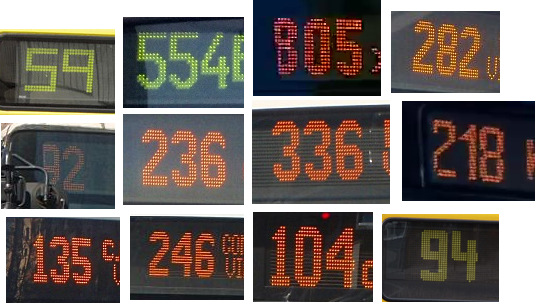
\includegraphics[width=0.5\textwidth]{img/number_test_sample}
	\caption{Przykładowe obrazy ze zbioru 6656 numerów linii autobusowych}
	\label{fig:number_test_sample}
\end{figure}

Jedna z~pierwszych prób przygotowania jak najlepszych 
detektorów cyfr zakładała (jak poprzednio)
półautomatyczne przygotowywanie zestawów zdjęć uczących. Pierwszy
zestaw przygotowywano w~pełni ręcznie, podczas gdy
elementy kolejnych zbiorów wybierano na podstawie
wyników detektora nauczonego z~wykorzystaniem zbioru 
z~poprzedniej iteracji. Próbowano w~ten sposób
korygować na bieżąco obserwowane tendencje do błędów.
Podejście, które sprawdziło się w~poprzednich dwóch przypadkach - 
podczas uczenia detektorów frontów i~numerów - 
powinno być adekwatne i~w~tym przypadku, szczególnie, że
podczas całego procesu możliwe byłoby dostrzeżenie tendencji
detektorów do wykrywania cyfr nieznacznie tylko od siebie różnych, takich jak
na przykład 6,8,9; 3,8; lub 7;2 oraz odpowiednia reakcja, czyli
umieszczanie takich przypadków z~zbiorze próbek negatywnych.


\begin{figure}[h!]\centering
	\begin{subfigure}{.55\linewidth}\centering
		\centering
		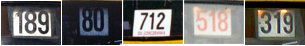
\includegraphics[width=1\textwidth]{img/usunieteNumery/stare}
		\caption{Tabliczki drukowane starego typu, nie uwzględnione
			w~założeniach}
	\end{subfigure}
	\hfill	
	\begin{subfigure}{.55\linewidth}\centering
		\centering
		
\includegraphics[width=1\textwidth]{img/usunieteNumery/przeswietlone}
		\caption{Obrazy prześwietlone}
	\end{subfigure}
	\hfill	
	\begin{subfigure}{.55\linewidth}\centering
		\centering
		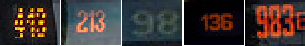
\includegraphics[width=1\textwidth]{img/usunieteNumery/rozdzielczosc}
		\caption{Mała rozdzielczość przechowywanych obrazów}
	\end{subfigure}
	\caption{Zdjęcia usunięte ze względu na znikomą przydatność i~poczynione
		założenia}
	\label{fig:removedNumbersCauseDamagedSkipped}
\end{figure}

Jednak podczas pracy ujawnił się zgoła inny problem.
Chodziło o~zniekształcenia i~defekty obrazów źródłowych takie
jak refleksy, przeszkody zasłaniające numer, uszkodzone lub migoczące
(podświetlone jedynie częściowo) wyświetlacze itp.
Problemy tego typu oczywiście brano pod uwagę, niepokojącą
była natomiast skala zjawiska.
Kilka przykładowych klas problemów zaprezentowano na rysunku
zbiorczym \ref{fig:removedNumbersCuseDistortion}.

\begin{figure}[h!]\centering
	\begin{subfigure}{.6\linewidth}\centering
		\centering
		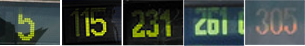
\includegraphics[width=1\textwidth]{img/usunieteNumery/cien}
		\caption{Cień padający na wyświetlacz}
	\end{subfigure}
	\hfill	
	\begin{subfigure}{.60\linewidth}\centering
		\centering
		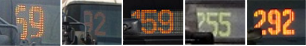
\includegraphics[width=1\textwidth]{img/usunieteNumery/lusterko}
		\caption{Lusterko boczne
			zasłaniające część wyświetlacza}
	\end{subfigure}
	\hfill	
	\begin{subfigure}{.60\linewidth}\centering
		\centering
		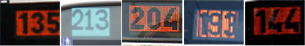
\includegraphics[width=1\textwidth]{img/usunieteNumery/negatyw}
		\caption{Numer linii prezentowany w negatywie}
	\end{subfigure}
	\hfill	
	\begin{subfigure}{.60\linewidth}\centering
		\centering
		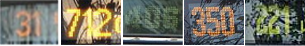
\includegraphics[width=1\textwidth]{img/usunieteNumery/odblask}
		\caption{Odblaski w przedniej szybie chroniącej wyświetlacz}
	\end{subfigure}
	\hfill	
	\begin{subfigure}{.60\linewidth}\centering
		\centering
		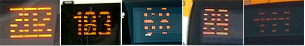
\includegraphics[width=1\textwidth]{img/usunieteNumery/paski}
		\caption{Wyświetlanie numeru w postaci zestawu poziomych pasów}
	\end{subfigure}
	\hfill	
	\begin{subfigure}{.60\linewidth}\centering
		\centering
		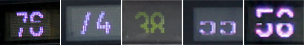
\includegraphics[width=1\textwidth]{img/usunieteNumery/wady}
		\caption{Uszkodzone wyświetlacze}
	\end{subfigure}
	\caption{Przykłady klas niezaadresowanych problemów}
	\label{fig:removedNumbersCuseDistortion}
\end{figure}

Wspomniane trudne przypadki to tylko część zlokalizowanych klas 
problemów. W~procesie przygotowania uniwersalnego i~niezawodnego czytnika numerów
nadjeżdżających autobusów wszystkie powyższe sytuacje powinny być
w~jakiś sposób rozwiązane i~odpowiednio obsłużone.

Osobnym wątkiem było czyszczenie zbioru z~elementów nieprzydatnych:
celowo pominiętych lub zepsutych, takich jak: numery linii w~postaci tabliczek drukowanych, zdjęcia prześwietlone, czy w~zbyt niskiej rozdzielczości. 
Przykłady usuniętych zdjęć,
które nie powinny wystąpić podczas rzeczywistej sesji odczytu numeru przedstawiono
na rysunku \ref{fig:removedNumbersCauseDamagedSkipped}

Na rysunku \ref{fig:removeAllCross} przedstawiony 
został przekrojowy podzbiór obrazów jakie usunięto ze zbioru 
testowego. Poza omówionymi już przypadkami, usuwano też
zdjęcia o~słabym kontraście spowodowanym równomiernym odblaskiem lub 
niską jasnością wyświetlacza. Natrafiono też na kilka przypadków zakłóceń
w~postaci opadów atmosferycznych - śnieg na obrazie w~prawym dolnym rogu na 
rysunku \ref{fig:removeAllCross}.


\begin{figure}[!h]
	\centering
	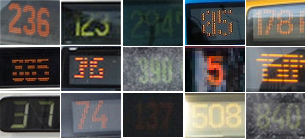
\includegraphics[width=0.6\textwidth]{img/usunieteNumery/rozne}
	\caption{Przekrojowy zestaw usuniętych numerów}
	\label{fig:removeAllCross}
\end{figure}

Dopiero po uświadomieniu sobie 
skali problemu - głównie mając na myśli odblaski 
i~problem z~częstotliwością odświeżania wyświetlacza - podjęto
kroki, które ostatecznie zaowocowały decyzją
o~przygotowaniu i~wykorzystaniu jedynie detektorów cyfr
i~rezygnacji z~wykorzystania wzorców w~celu weryfikacji/potwierdzenia
wykrytych obszarów. 

Kolejnym - nawet bardziej istotnym - 
problemem, który pojawił się na etapie dopasowywania wzorca
była błędna klasyfikacja cyfr na przykładzie fragmentu obrazu oznaczonego
przez detektory cyfr 6 i~8.
Obiekt zainteresowania przedstawiał cyfrę 8, jednak 
wyliczanie podobieństwa dla zadanego
obszaru i~przygotowanych wzorców wskazywało większą wartość dla
wzorca reprezentującego cyfrę 6. 
Co gorsza, klasyfikacja pozostała błędna nawet gdy wzorzec dla cyfry 8 przygotowano na podstawie tego właśnie konkretnego obrazu.
Powodem mogły być manipulacje na obrazie wykonywane podczas procesu dopasowania.
Wzorce były bowiem przeskalowywane do kilku zadanych rozmiarów. Mogło to wprowadzić pewne zniekształcenia i~zaburzenia w~ocenie, tym niemniej
był to kontrprzykład uniemożliwiający wykorzystanie wymienionej techniki w~rozwiązaniu
końcowym. 

Użyty mechanizm został opisany na końcu kolejnego podrozdziału. Głównym założeniem
niezbędnym do przeprowadzenia poprawnego odczytu było posiadanie co najmniej kilku
obrazów przedstawiających numer linii autobusowej. Dla takiego zbioru
miejsca najczęściej oznaczane przez detektory cyfr - jeszcze bez podziału na typ -
były opisywane odpowiednią cyfrą poprzez wyłonienie detektora, który miał największy 
procentowy udział na przestrzeni kilku ujęć. 

\subsection{Symulowane przypadki użycia}

Na podstawie pięciu filmów nagranych przy pomocy telefonu wykonano pięć
symulowanych sesji wykrywania frontu nadjeżdżającego autobusu.
Wycinane i~zapisywane były fronty autobusów oraz fragmenty
reprezentujące numer linii autobusowej. Pojedyncze 
elementy dla pięciu przypadków przedstawiono 
na rysunku \ref{fig:5usecasesOverall}.

\begin{figure}[!h]
	\centering
	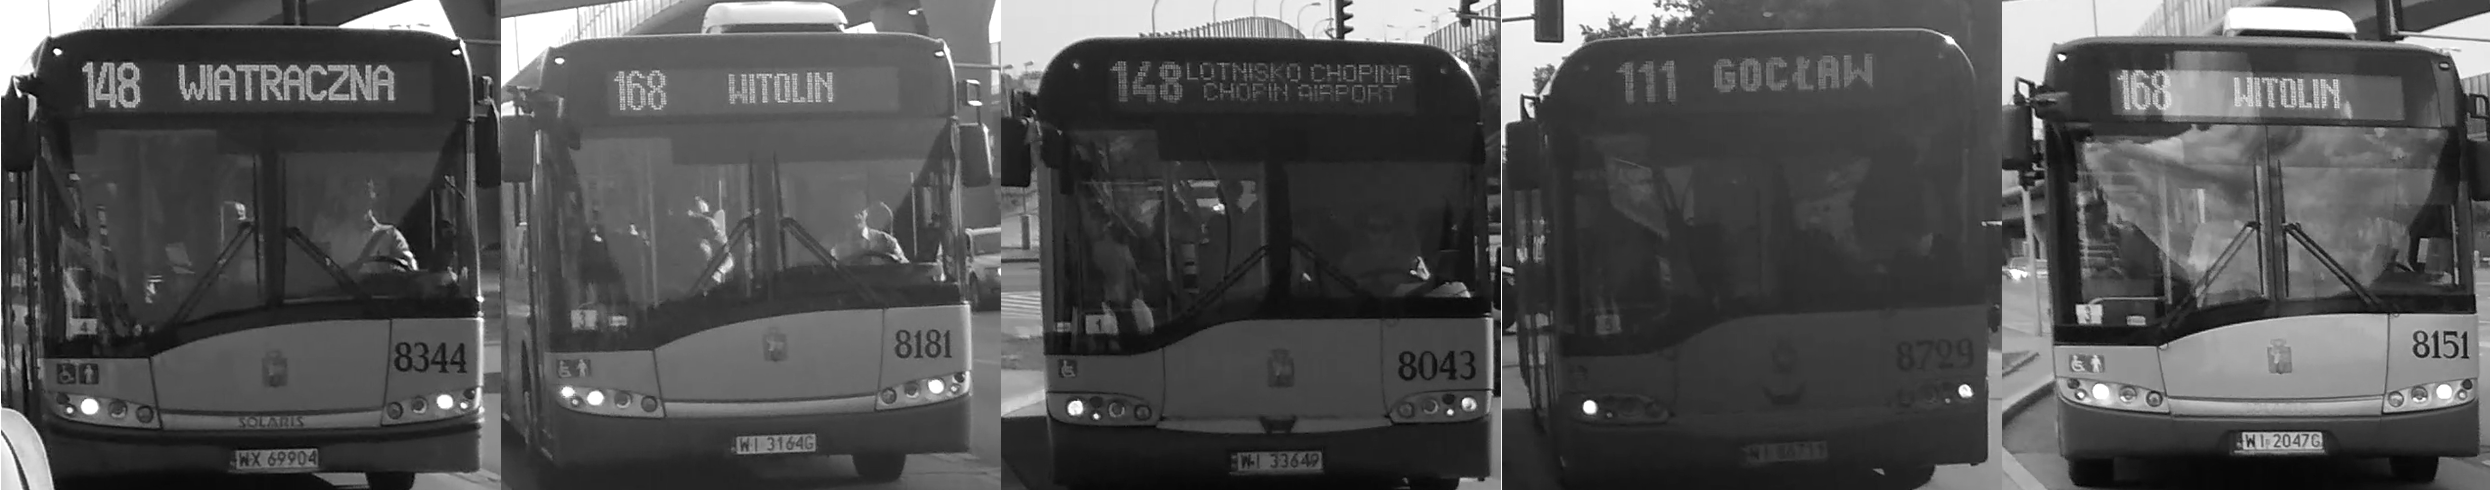
\includegraphics[width=1.01\textwidth]{img/5sessions/overall}
	\caption{Przykłady wycinków frontów z~pięciu sesji detekcji}
	\label{fig:5usecasesOverall}
\end{figure}

Statystyki poszczególnych sesji zamieszczone zostały w~tabeli
\ref{tab:5usecasesStats}. Jak widać detektory frontów
były raczej stabilne, wystarczająco skuteczne i~odporne 
na błędy. Co prawda w~drugim wierszu - dla numeru 168 (bez odblasków)
- odnotowano poważną liczbę błędów, to nadal jest to 
mniej niż połowa wszystkich oznaczeń w~sesji. Dodatkowo
na~drugim etapie weryfikacji - detekcja numeru linii - błędnie 
wyznaczone fragmenty zostały odrzucone poprzez 
nieodnalezienie w~nich fragmentu
z~numerem linii autobusowej. Co ciekawe dla tego
przypadku osiągnięto najmniejszy odsetek błędów
podczas owego drugiego etapu. 

\begin{table}[!h]
	\centering                                                          
	\caption{Statystiki pięciu sesji testowych}
	\begin{tabular}{r|r|l|r|l}
		Front    & Liczba poprawnie     & Liczba błędów  & Liczba poprawnie   & Liczba błędów     \\
		         & wykrytych frontów    & (fronty)        & wykrytych numerów  & (numery)  \\
		\hline
		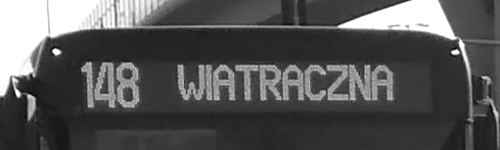
\includegraphics[width=0.15\textwidth]{img/5sessions/01-148} & 116 & 4 & 116 & 28 \\
		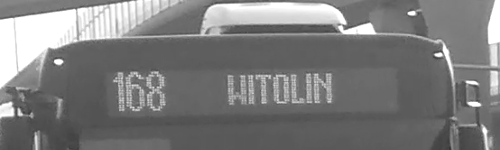
\includegraphics[width=0.15\textwidth]{img/5sessions/02-168} & 151 & 40 & 105 & 1 \\
		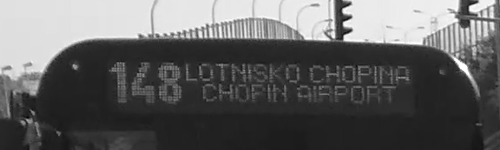
\includegraphics[width=0.15\textwidth]{img/5sessions/03-148} & 171 & 0 & 108 & 3  \\
		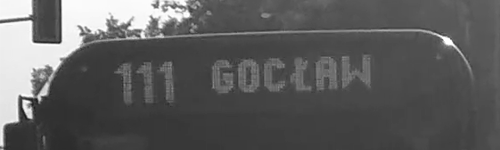
\includegraphics[width=0.15\textwidth]{img/5sessions/04-111} & 93  & 0 & 50 & 19 \\
		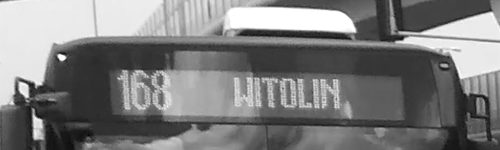
\includegraphics[width=0.15\textwidth]{img/5sessions/05-168} & 203 & 0 & 128 & 30 \\
	\end{tabular} 
	\label{tab:5usecasesStats}
\end{table}

Fragmenty obrazów błędnie wskazane jako fronty autobusów zostały przedstawione i~opisane na rysunku \ref{fig:5usecasesFrontErrorSamples}.
Pracując nad poprawieniem skuteczności detekcji oraz
zmniejszeniem liczby błędów można by dodać obrazy te do zbioru
obrazów negatywnych użytych podczas uczenia detektorów.
Drugim, prostszym rozwiązaniem byłaby zmiana parametru -
\verb|minNeighbours| - zadanego podczas wywołania detektora.
Do tej pory wartość tego parametru była ustawiona na 1. Zwiększenie
wartości powinno spowodować spadek liczby błędów, kosztem
spadku poprawnych wykryć. Warto jednak zauważyć, że 
w~żadnym błędnie oznaczonym fragmencie nie został wykryty 
fragment potencjalnie reprezentujący numer. Co znaczy, że problem można
na tym etapie zignorować. Ostatecznie preferowanym rozwiązaniem byłoby
dodanie błędnie oznaczonych fragmentów do zbioru obrazów negatywnych.

\begin{figure}[h!]\centering
	\begin{subfigure}{.24\linewidth}\centering
		\centering
		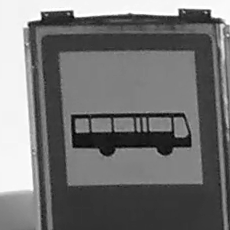
\includegraphics[width=1\textwidth]{img/5sessions/01-wrong-01}
		\caption{4 w~pierwszym i~8~w~drugim zbiorze}
	\end{subfigure}
	\hfill	
	\begin{subfigure}{.24\linewidth}\centering
		\centering
		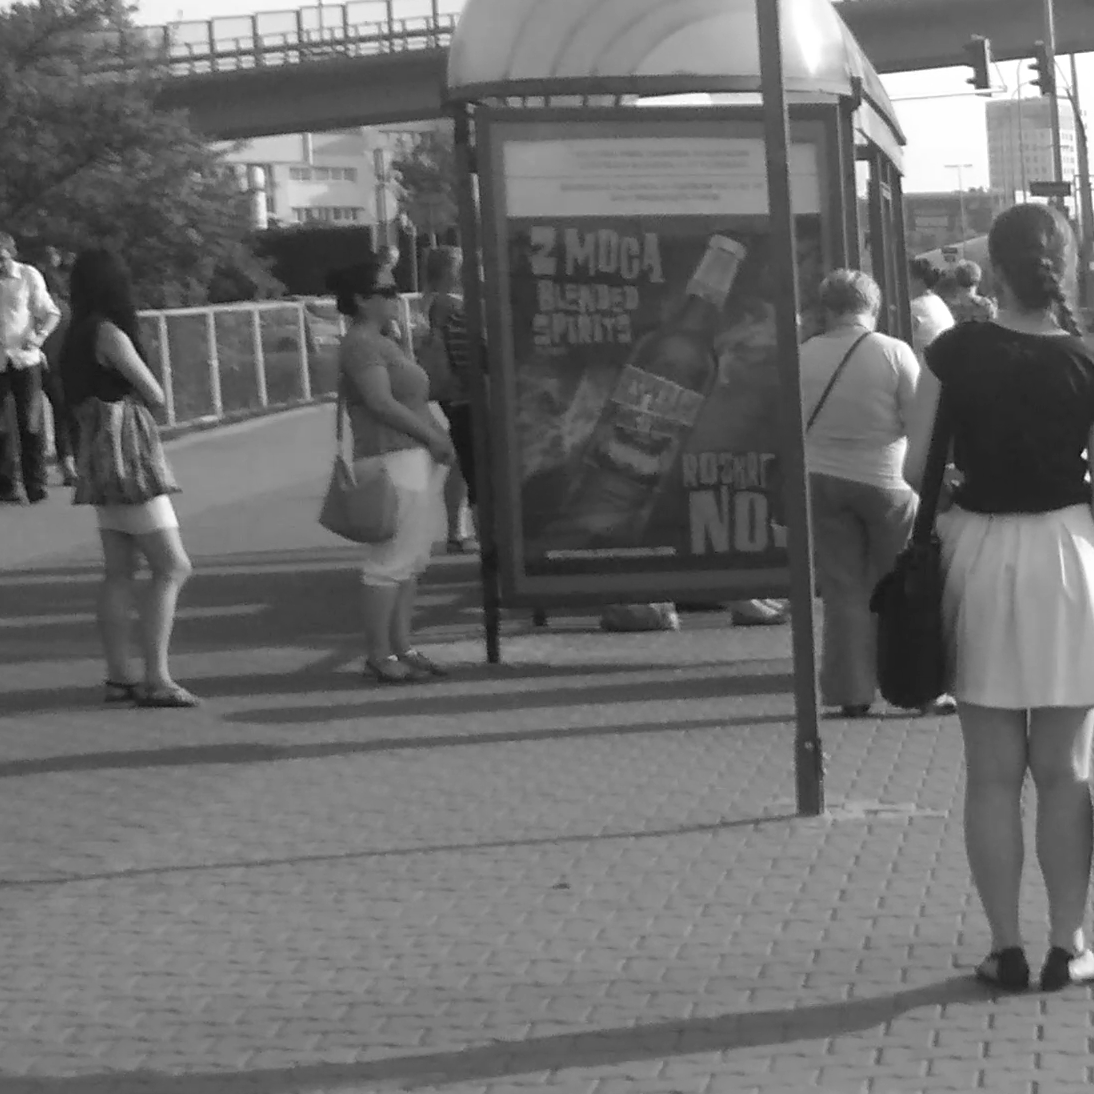
\includegraphics[width=1\textwidth]{img/5sessions/02-wrong-05}
		\caption{24 wystąpienia w drugim zbiorze}
		\label{img:local5sessionsGroup}
	\end{subfigure}
	\hfill	
	\begin{subfigure}{.24\linewidth}\centering
		\centering
		\includegraphics[width=1\textwidth]{img/5sessions/02-wrong-03}
		\caption{jeden fragment z~elementów \ref{img:local5sessionsGroup}}
		\label{img:local5sessionsGroup2}
	\end{subfigure}
	\hfill	
	\begin{subfigure}{.24\linewidth}\centering
		\centering
		\includegraphics[width=1\textwidth]{img/5sessions/02-wrong-02}
		\caption{dwa fragmenty z~obrazów \ref{img:local5sessionsGroup} i~\ref{img:local5sessionsGroup2}}
	\end{subfigure}
	\hfill	
	\begin{subfigure}{.24\linewidth}\centering
		\centering
		\includegraphics[width=1\textwidth]{img/5sessions/02-wrong-04}
		\caption{jeden podobraz fragmentu \ref{img:local5sessionsGroup2}}
	\end{subfigure}
	\hfill	
	\begin{subfigure}{.24\linewidth}\centering
		\centering
		\includegraphics[width=1\textwidth]{img/5sessions/02-wrong-06}
		\caption{pojedynczy obraz z~drugiego zbioru}
	\end{subfigure}
	\hfill	
	\begin{subfigure}{.24\linewidth}\centering
		\centering
		\includegraphics[width=1\textwidth]{img/5sessions/02-wrong-07}
		\caption{pojedynczy obraz z~drugiego zbioru}
	\end{subfigure}
	\hfill	
	\begin{subfigure}{.24\linewidth}\centering
		\centering
		\includegraphics[width=1\textwidth]{img/5sessions/02-wrong-01}
		\caption{pojedynczy obraz z~drugiego zbioru}
	\end{subfigure}
	\caption{Przykłady błędnie wyznaczonych frontów}
	\label{fig:5usecasesFrontErrorSamples}
\end{figure}

Trudniejszym do rozwiązania problemem było oznaczanie fragmentów 
tekstu reprezentującego opis miejsca docelowego kursu jako numeru
linii. Najczęstsze przypadki 
przedstawiono na rysunku \ref{fig:5usecasesNumberErrorSamples}.
Drugi obrazek reprezentuje sytuację najmniej szkodliwą. 
Ostatecznie jest to przecież fragment w~którym powinien
być numer linii. Obraz został pobrany w~momencie całkowitego
wygaszenia wyświetlacza. Dodatkowo żaden detektor cyfr nie powinien 
oznaczyć tutaj żadnego fragmentu obrazu jako cyfry. Sytuacja ma się gorzej
w~trzech pozostałych przypadkach. Mogą one wprowadzać zaburzenia poprzez dodawanie
błędnych odczytów, do zbioru. Prostym, acz skutecznym rozwiązaniem było ograniczenie
pola przeszukiwań do lewego górnego obszaru frontu autobusu
o~zadanych wymiarach. Dzięki temu usunięto błędne
oznaczenia, przy zachowaniu pozytywnych.

\begin{figure}[h!]\centering
	\begin{subfigure}{.4\linewidth}
		\centering
		\includegraphics[width=0.3\textwidth]{img/5sessions/01-numwrong-01}
		\caption{28 sztuk w~zbiorze pierwszym}
	\end{subfigure}
	\hfill	
	\begin{subfigure}{.4\linewidth}
		\centering
		\includegraphics[width=.3\textwidth]{img/5sessions/02-numwrong-01}
		\caption{1, 3, 11 odpowiednio w~2, 3 i 5 zbiorze}
	\end{subfigure}
	\hfill	
	\begin{subfigure}{.4\linewidth}
		\centering
		\includegraphics[width=0.3\textwidth]{img/5sessions/04-numwrong-01}
		\caption{19 sztuk w~zbiorze czwartym}
	\end{subfigure}
	\hfill	
	\begin{subfigure}{.4\linewidth}
		\centering
		\includegraphics[width=0.3\textwidth]{img/5sessions/03-numwrong-01}
		\caption{19 sztuk w~zbiorze piątym}
	\end{subfigure}
	\caption{Przykłady błędnie wyznaczonych frontów}
	\label{fig:5usecasesNumberErrorSamples}
\end{figure}

Przypadek piąty - linia 168 (z~odblaskami) - był przedstawicielem sytuacji
najtrudniejszej z~omawianych. Nakładały się tu dwa problemy: dużo pustych
fragmentów, które powinny przedstawiać numer oraz odblaski.
Puste fragmenty obrazów spowodowane były efektem migotania wyświetlacza.
Diody zapalały się z~tak niewielką częstotliwością, że aparat telefonu
pobierając obrazy natrafiał na sceny, w~których wyświetlacz był całkowicie
lub częściowo wygaszony. Przykład takich sytuacji przedstawiono na rysunku
\ref{fig:5usecasesFlickeringProblem}. Wszystkie opisane, problematyczne 
fragmenty reprezentujące numer zostały usunięte przed przejściem do następnego kroku,
czyli próby przygotowania algorytmu odczytującego numer linii autobusowej - ostatniego
kroku proponowanej kaskady.

\begin{figure}[!h]
	\centering
	\includegraphics[width=0.8\textwidth]{img/5sessions/flickering168/out}
	\caption{Problem z~niską częstotliwością odświeżania wyświetlacza - klatki
		uchwycone w~trakcie odświeżania lub zupełny brak numeru}
	\label{fig:5usecasesFlickeringProblem}
\end{figure}

Przygotowano 10 detektorów cyfr o~wymiarach 20 na 30 pikseli (pionowy prostokąt).
Podczas procesu uczenia wykorzystano domyślne wartości narzędzia 
\verb|opencv_traincascade|. 
Podkręcono jedynie oczekiwany odsetek pozytywnych trafień z~domyślnej wartości:
0.995 na 0.999. Dla poszczególnych cyfr wykorzystano następujące liczby 
próbek pozytywnych i~negatywnych:
\begin{itemize}
	\item 0 - 300/600 (pos/neg),
	\item 1 - 600/1200,
	\item 2 - 500/1000,
	\item 3 - 600/1200,
	\item 4 - 450/900,
	\item 5 - 400/800,
	\item 6 - 300/600,
	\item 7 - 180/360,
	\item 8 - 350/700,
	\item 9 - 320/640.
\end{itemize}

Było to podyktowane głównie tym, że takie liczby wycinków
obrazów reprezentujących poszczególne cyfry przygotowano na samym początku
prac i~dodatkowe oznaczanie - ze~względu na czasochłonność - nie wchodziło już w~rachubę.

Zbiór negatywów przygotowano automatycznie poprzez wybranie
numerów nie zawierających szukanej cyfry ze zbioru wykorzystanego
na etapie uczenia detektora numerów jak na rysunku \ref{fig:number_test_sample}.
Numer widoczny na obrazie był zapisany również w~nazwie pliku co
ułatwiło napisanie stosownego narzędzia. Zbiór negatywny składał
się z~obrazów reprezentujących całe numery, nie zawierające zadanej cyfry.
Czyli dla 0 byłyby to numery 1,2,(...),991,992,(...),999. Liczba negatywnych
próbek była podyktowana chęcią zachowania stosunku 1:2 - pozytywów do negatywów.

\subsubsection{Test na liczbę wykrytych cyfr w~numerze (bez lokalizacji)}

Jako ostatni wykonany został bardzo prosty test, mający na celu zliczenie
wszystkich wykryć - pozytywnych i~negatywnych - z~podziałem na 
poszczególne detektory cyfr.
Danymi wejściowymi były sekwencje obrazów
opisane w~poprzednim podrozdziale. Wykorzystano wycinki reprezentujące numery linii autobusowych, których przykłady przedstawiono na rysunku \ref{fig:sample_last_input_numbers}.

\begin{figure}[!h]
	\centering
	\includegraphics[width=0.9\textwidth]{img/5sessions/part2-overall}
	\caption{Przykłady wycinków numerów z~pięciu sesji detekcji. Liczebność poszczególnych
		zbiorów (w~kolejności z~rysunku): 168(z~odblaskami):128, 168(bez odblasków):105, 148(cienka czcionka):116, 148(gruba czcionka):108, 111:50}
	\label{fig:sample_last_input_numbers}
\end{figure}

Dla każdej z~przedstawionych sekwencji obrazów uruchomiono detektory cyfr od 0 do 9.
Sumaryczną liczbę wykryć przedstawiono w~tabeli \ref{tab:5usecasesStatsNumbers}.

\begin{table}[!h]
	\centering                                                          
	\caption{Liczba wykryć poszczególnych cyfr w~pięciu sesjach testowych, dla 
		numerów: 148, 168, 148, 111 i 168}
	\begin{tabular}{r|c|c|c|c|c|c|c|c|c|c|l}
		\diag{0.5em}{1.5cm}{Numer}{Detektor} & 0 & 1 & 2 & 3 & 4 & 5 & 6 & 7 & 8 & 9 & Liczba obrazów   \\
		\hline
		\includegraphics[width=0.05\textwidth]{img/5sessions/01-148-number} & 3 & \textbf{105} & 2 & 13 & \textbf{108} & 0 & 1 & 0 & \textbf{93} & 1 & 108  \\
		\includegraphics[width=0.05\textwidth]{img/5sessions/02-168-number} & 18 & \textbf{103} & 2 & 10 & 10 & 8 & \textbf{118} & 3 & \textbf{99} & 8 & 105  \\
		\includegraphics[width=0.05\textwidth]{img/5sessions/03-148-number} & 24 & \textbf{136} & 0 & 14 & \textbf{118} & 1 & \underline{75} & 0 & \textbf{117} & 23 & 116  \\
		\includegraphics[width=0.05\textwidth]{img/5sessions/04-111-number} & 0 & \textbf{154} & 0 & 0 & 0 & 0 & 0 & 1 & 0 & 0 & 50  \\
		\includegraphics[width=0.05\textwidth]{img/5sessions/05-168-number} & 25 & \textbf{126} & 2 & 14 & 14 & 4 & \textbf{128} & 0 & \textbf{109} & 5 & 128  \\
	\end{tabular} 
	\label{tab:5usecasesStatsNumbers}
\end{table}

Gdyby nie wynik uzyskany 
dla detektora cyfry sześć dla numeru 148 (tego wyświetlanego przy użyciu 
czcionki grubszej) problem
można by uznać za rozwiązany. Tym niemniej dane z~tabeli 
\ref{tab:5usecasesStatsNumbers} wykazały, że żadne dodatkowe
działania w~postaci dopasowywania wzorców nie będą potrzebne. 
Ponadto podczas wstępnych prób z~metodą \verb|template matching| osiągnięto rezultaty
poniżej oczekiwanych. Metoda ta okazała się trudna w~poprawnej implementacji,
kosztowna obliczeniowo i~w~omawianym przypadku bardzo zawodna.

Wykorzystując fakt, że podczas jednej sesji rozpoznawania numeru 
linii dysponujemy więcej niż jednym obrazem frontu autobusu 
sporządzono algorytm, który na podstawie oznaczeń wszystkich
detektorów cyfr wyznacza potencjalne miejsce (i~liczbę) cyfr
w~obrazie, a~następnie dla wyznaczonych miejsc (mapa w~której kluczem 
są wartości współrzędnej x) wybiera tę cyfrę, której detektor oznaczył 
największą liczbę wystąpień.

Powyższe podejście poza niezaprzeczalną szansą na powodzenie, 
 rozwiązuje dodatkowo problemy z~częstotliwością odświeżania
wyświetlacza - sytuację gdy numer jest zupełnie niewidoczny podczas
jego wygaszenia. Istnieje też szansa na zmniejszenie negatywnego
wpływu odblasków na skuteczność - 
poprzez ciągłe pobieranie obrazów do analizy autobus może przez 
chwilę znaleźć się w~takim położeniu, że wyświetlacz będzie dobrze widoczny, bądź
kolejno, wraz z~upływem czasu dobrze widoczne będą poszczególne cyfry numeru.
Potrzebne jest jednak wiele pracy na zweryfikowanie w~jakim stopniu poprawia
to ogólną skuteczność programu w~trudnych warunkach oświetleniowych.

W~kolejnym rozdziale wykonano kilka testów wydajnościowych
na urządzeniu. Zmierzono czasy wykonania poszczególnych elementów 
systemu oraz podjęto próby wskazania słabych jego fragmentów -
tak zwanych wąskich gardeł.